% Payload-Aware Two-Tier UAV Route Planning — Review II Report

\documentclass{ssnreview}

\usepackage{amsmath}
\usepackage{amsfonts}
\usepackage{amssymb}
\usepackage[numbers]{natbib}
\usepackage{xltabular}
\usepackage{multirow}
\usepackage{algorithm}
\usepackage{algpseudocode}
\usepackage{listings}
\usepackage{xurl}                     % break long URLs anywhere (bib underfull/overfull)
\setlength{\emergencystretch}{2em}    % last-resort stretch, kills stray over/underfull hboxes
\bibliographystyle{unsrtnat}
\graphicspath{{../diagrams/}{figures/}}
\newcommand{\doi}[1]{doi: \href{https://doi.org/#1}{#1}}
\newcommand{\flowchapter}[1]{\par\addvspace{30pt}\let\origclearpage\clearpage\let\clearpage\relax\chapter{#1}\let\clearpage\origclearpage}  % no group: \label after it gets the chapter number
\lstset{basicstyle=\ttfamily\footnotesize, keywordstyle=\color{blue!60!black}\bfseries,
  commentstyle=\color{gray}, stringstyle=\color{teal}, frame=single, breaklines=true,
  showstringspaces=false, columns=fullflexible, captionpos=b}
\renewcommand{\lstlistingname}{Listing}

\projecttitle{PAYLOAD-AWARE TWO-TIER UAV ROUTE PLANNING FOR LAST-MILE DELIVERY}
\reviewnumber{REVIEW REPORT -- II}
\students{%
  Thirumurugan RA \hfill (3122235001149)\\
  Meghna Manimaran \hfill (3122235001079)\\
  Shrika SP Thota \hfill (3122235001125)}
\supervisor{Dr. N. Sujaudeen, Assistant Professor}
\department{Department of Computer Science and Engineering}
\institution{Sri Sivasubramaniya Nadar College of Engineering}
\academicyear{2026--2027}
\collegelogo{ssn-logo.png}

\begin{document}
\makereviewtitle
\reviewfrontmatter

% ============================================================
\begin{reviewabstract}
In UAV systems for medical and emergency last-mile delivery, conflicting objectives
must be balanced: higher flight risk is carried by shorter routes, more battery is
drained by low-risk corridors, and the fastest paths are rarely achieved by
energy-efficient routing. No single fixed trade-off serves all payload types, yet the
same objective weights are applied by existing planners to every mission regardless of
the payload. In existing multi-objective planners, including entropy-based, diversity-driven, and
crowding-distance Pareto selection methods, objective weights are encoded as a fixed
scalar before path search begins. No influence is exerted by payload properties such as
fragility class, payload weight class, and delivery urgency over which Pareto-optimal
route is chosen. When payloads change, weights must be manually re-tuned and planners
re-run by operators, which is unworkable under field conditions. The proposed work is a Payload-Aware Two-Tier UAV Route Planning system, wherein
Pareto front construction is separated from route selection and an explicit algebraic
bridge is added between Tier 1 routing objectives and Tier 2 payload metadata.
In Tier 1, a multi-objective A*/Dijkstra graph-search is executed over an OpenStreetMap
airspace graph, producing a Pareto-optimal route set across distance, energy
consumption, and flight risk. In Tier 2, four operator-assigned payload tags are read
and objective weights derived: $w_\mathrm{risk}$ is scaled by fragility class,
$w_\mathrm{distance}$ by delivery urgency, and $w_\mathrm{energy}$ by payload weight
class. Every Pareto point is scored by these weights via a utility function, and the
argmax is selected as the mission route. Evaluation will be conducted on synthetic
graphs (50, 200, 500 nodes) against single-objective A* and MOPSO baselines using
hypervolume, spread, and Tier 2 accuracy. Hardware validation will use a Pixhawk
quadcopter via ArduPilot SITL simulation and outdoor flights. Planned experiments will quantify Tier 1 gains over both baselines, evaluating whether
non-extreme Pareto points are selected for mixed-priority payloads. The principal contribution is a formula-driven mapping from metadata to routing weights,
linking mission context directly to Pareto selection without expert intervention. Route
choice is set by payload properties rather than context-blind diversity criteria. The
Pareto front is rebuilt periodically, serving all missions between updates.

\keywords{UAV route planning; multi-objective optimisation; NAMOA*; Pareto front; payload-aware selection; wind-aware risk; last-mile delivery}
\end{reviewabstract}

% ============================================================
\chapter{Introduction}\label{cha:intro}

Unmanned aerial vehicles (UAVs) are a useful platform for last-mile delivery in
scenarios where ground transport is impractical: medical supply chains to remote
clinics, emergency drug drops during disaster response, and fragile diagnostic sample
transport where road vibration risks contamination. In each scenario the UAV must
fly a route from a dispatch hub to a delivery point across an airspace that contains
obstacles, regulated no-fly zones, and variable wind corridors. A good route balances
three conflicting objectives: total flight distance, battery energy use, and exposure to
high-risk segments.

This three-way conflict is exactly what multi-objective UAV path planning is built to
handle. Rather than collapsing distance, energy, and risk into one score before the
search runs, a multi-objective planner keeps all three objectives separate through the
search and returns a Pareto-optimal front: a set of routes where none can be improved on
one objective without giving up ground on another \cite{r11}. The front tells the
operator what trade-offs are available; it does not, by itself, say which route to fly.

One common way to sidestep the trade-off question is to form a weighted sum of the
three objectives into a single scalar cost function and then run a conventional path
planner such as A* on it. This scalar collapses the multi-objective problem into a
single-objective one, and the operator adjusts the three weights to express the
mission's priority before each flight. The approach works for a fixed mission type, but
it fails immediately when the payload changes: emergency medicine requires a completely
different weight profile from fragile biological samples or disaster-relief bulk
supplies \cite{r1}. Manually re-tuning and re-running the planner between missions is
operationally impractical in time-critical field conditions.

\section{Background}

Building the Pareto front, as introduced in Chapter~\ref{cha:intro}, is well studied:
the field has produced graph-search and population-based methods that generate
well-spread, non-dominated route sets efficiently. The question that decides whether
any such system is useful in practice is how the
final route gets picked from the front. Section~\ref{sec:relatedwork} reviews three
directly relevant papers and finds the same answer in each: delivery context plays no
role. None of them let what the UAV is carrying influence route choice, or even ask
which route should be chosen for a given payload. That is the gap this project
addresses.

Autonomous UAV systems for medical and emergency last-mile delivery work under a
constraint that separates them from general routing problems: the best route trade-off
changes with the payload. A fragile diagnostic sample needs a low-vibration,
low-turbulence corridor even at the cost of a much longer flight time. Emergency insulin
needs the shortest path regardless of risk. Bulk disaster-relief supplies need the most
energy-efficient route to maximise delivery range.

Payload-awareness itself is not absent from the UAV literature: variable payload mass has
been used to adapt the flight-speed and energy-consumption \emph{model itself} during
trajectory planning, recomputing the underlying physical equations as mass changes across
a multi-drop mission \cite{r10}. What is absent is any use of payload metadata to
\emph{select} a point on a pre-computed multi-objective Pareto front. Tier~2's payload
weight tag is a discrete, ordinal class (light/medium/heavy) that is one of four metadata
tags algebraically blended into a static selection weight once per mission; it never
alters the per-edge energy model or triggers re-planning, unlike \cite{r10}'s continuous
mass-driven physics adaptation. Tier~2 closes that gap by selecting among a fixed front
from metadata, rather than adapting the model to continuous mass.

Real deployments show where payload matters, and how thin the public evidence still is.
Swiss Post flew laboratory samples between hospitals on Matternet quadrotors until two
incidents in 2019 led it to suspend the service. In January a short circuit cut power to
the GPS and the drone made an emergency landing on Lake Z\"{u}rich. In May a parachute
tether snagged on the airframe and the 22-pound drone fell into woods near a group of
kindergarten children~\cite{r12}. Both were equipment failures, so they say nothing
about route choice. They do show that lab samples are flown over water and populated
ground, where the choice of corridor has consequences.

The laboratory evidence on how sensitive these payloads are is mixed. Drone vibration is
real: in-flight levels exceeded road transport by up to a factor of three, at much higher
frequencies, yet insulin flown on fixed-wing and multi-copter drones showed no
aggregation~\cite{r13}. Sixty flights carrying monoclonal antibody infusions, with
vibration between 1.5 and 3\,g, left particle size and aggregation unchanged~\cite{r14}.
A blood-sample study found drone transport comparable to car transport, with small
differences in five of the analytes tested~\cite{r15}. The tested payloads survived
ordinary flights. None of the three studies varied the route, so they cannot say whether
a smoother corridor would protect a more fragile cargo. In this work the fragility tag is
therefore a precaution the operator sets, not a degradation effect measured in the
literature.

Zipline's blood-delivery network in Rwanda serves hospitals up to about 80\,km from its
distribution centre, and each aircraft follows a predetermined flight plan~\cite{r16}.
Its engineers treat payload weight as a limit on range. That is the energy side of the
problem Tier~2 addresses: a heavier load shortens how far the drone can go, so the best
route depends on what is aboard.

\section{Motivation}

Three real operational scenarios motivate this work, and their routing requirements do
not agree.

Fragile medical samples such as tissue biopsies and blood specimens must arrive intact.
The studies cited in the Background found no damage on ordinary flights, but an operator will still want such a payload kept out of rough air. The routing priority
is to minimise flight risk, taken here as time spent in turbulent corridors, sudden
altitude changes, and wind-exposed segments. For this payload a route that is noticeably
longer but spends far less time in turbulent air is the better one.

Emergency medicine such as insulin or antivenom has a strict time window. The priority
is the shortest route, so transit time is lowest; flight risk and energy come second.
For a 15-minute delivery window, the shortest path wins outright.

Disaster-relief bulk supplies such as water purification tablets and ration packs are
heavier than medical payloads and are neither urgent nor fragile. The priority is the
lowest battery drain, so a single charge covers as many deliveries as possible.

No existing UAV planner switches between these three routing strategies from a payload
tag. The proposed two-tier system does this with no expert intervention and no
replanning. In the UAV delivery literature, payload metadata (fragility class, payload
weight class, delivery urgency) has never been the sole input to automatic Pareto point
selection. That is the gap this project targets.


\section{Related Work}\label{sec:relatedwork}

Multi-objective UAV path planning draws on both graph-search and evolutionary
optimisation \cite{r11}. Within it, route selection from a computed Pareto
front is usually guided by the crowding-distance rule introduced by NSGA-II \cite{r8},
or by an entropy criterion that keeps the archive diverse while a manually weighted
scalar sum makes the final pick; neither considers delivery context. Payload
information, where it appears at all, is limited to continuous mass folded directly into
the energy/speed model itself, not discrete metadata used to select among a pre-computed
Pareto front. Three papers most directly
relevant to the proposed work are reviewed below; Table~\ref{tab:related-work} gives a
structured comparison.

\small
\begin{xltabular}{\textwidth}{>{\centering\arraybackslash}p{1.1cm} L{2.9cm} Y Y Y}
\caption{Summary of related work}\label{tab:related-work}\\
\toprule
\textbf{S.No.} & \textbf{Author/Year} & \textbf{Proposed Method} & \textbf{Key Findings} & \textbf{Limitations}\\
\midrule
\endfirsthead
\multicolumn{5}{l}{\small\itshape Table \thetable\ (continued)}\\
\toprule
\textbf{S.No.} & \textbf{Author/Year} & \textbf{Proposed Method} & \textbf{Key Findings} & \textbf{Limitations}\\
\midrule
\endhead
\midrule
\multicolumn{5}{r}{\small\itshape continued on next page}\\
\endfoot
\bottomrule
\endlastfoot
1 & Chokkalingam \& Ganesan (2026) \cite{r1} &
Pareto-optimal particle swarm optimisation (POPSO) with dynamic parameter adaptation and
Pareto--entropy archive selection to maintain front diversity during optimisation; the
final single route is then read off via a weighted-sum scalarisation whose weights are
set empirically per mission. &
Entropy-guided archiving improves front diversity and adaptability to real-time
environmental changes over static-weight baselines. &
Final route choice still reduces to a manually re-tuned weighted sum per mission;
payload metadata never incorporated, so fragile samples and emergency medicine receive
the same hand-tuned selection procedure from the same front.\\[4pt]
2 & Tsoutsouras et al.\ (2020) \cite{r10} &
Adapts flight speed and the energy-consumption model to the UAV's instantaneous payload
mass during trajectory planning for multi-user delivery missions, updating the
trajectory as mass changes between drop-offs. &
Mass-aware trajectory adaptation reduces energy consumption relative to mass-agnostic
planning across multi-stop delivery routes. &
Uses continuous payload mass only as a physical parameter inside the energy/speed model
itself; builds no multi-objective Pareto front and has no notion of discrete payload
metadata (fragility class, payload-weight class, urgency) selecting among pre-computed
routing trade-offs.\\[4pt]
3 & Ren et al.\ (2019) \cite{r3} &
Crowding-distance-based NSGA-II (CDNSGA-II) for multi-objective UAV path planning,
balancing distance and safety over an octree-represented urban environment. &
CDNSGA-II finds well-spread, collision-free Pareto-optimal paths efficiently in
octree-modelled urban airspace. &
Crowding distance encodes only the geometric spread of the front; it cannot represent
urgency, fragility, or payload weight, and mission context plays no role in
selection.
\end{xltabular}
\normalsize

\section{Research Gap}\label{sec:gap}

Two of the three reviewed papers treat Pareto-front diversity as the central design
concern, and only one of those two uses it to \emph{select} a route: the crowding
distance of \cite{r3} picks a single point directly from the front, while \cite{r1} uses
entropy only to keep the archive \emph{diverse} during optimisation and falls back to a
manually weighted scalar sum, re-tuned per mission by a human operator, to make the
actual final pick. \cite{r10} does not build a Pareto front at all: it folds continuous
payload mass into the energy model's equations of motion and adapts flight speed as mass
changes across a multi-drop mission, but never selects among competing routing
trade-offs by payload. Whether the mechanism is geometric diversity or continuous
mass-driven physics adaptation, none of the three use payload weight, or any other
payload property, as a discrete input to a Pareto-point \emph{selection} mechanism; in
\cite{r10}, mass reshapes the cost model itself and never enters a selection formula.
This is the gap the proposed system closes: Tier~2 treats payload weight as one of four
ordinal metadata tags algebraically blended into a selection weight, and does not use it
as a continuous physical parameter inside the cost model.

The gap is not an implementation detail; it is a design assumption shared by all three
approaches. Entropy and crowding distance are both defined purely over the
geometry of the Pareto front; mass-aware trajectory adaptation is defined purely over the
physical energy model, with mass entering as a continuous parameter to that model, never
as a selection criterion. None of these mechanisms has an interface through which
discrete payload metadata, as opposed to continuous mass or point geometry, can enter a
\emph{selection} step. Adding payload information to them would mean replacing the
selection criterion outright, which is what the proposed Tier~2 utility scoring does.

This work addresses three specific gaps.

\begin{enumerate}[label=\textbf{Gap~\arabic*.}]
  \item Existing UAV multi-objective planners offer no payload-aware route selection:
  they apply a fixed geometric criterion independent of payload type, or no selection
  mechanism at all. Tier~2 maps four payload tags directly to Pareto point selection
  through a formula.
  \item Existing planners do not re-use one front across mission types; they re-run the
  full multi-objective search whenever the mission context changes. The two-tier
  separation decouples front construction from mission arrivals: Tier~1 refreshes the
  front on a periodic cadence, independent of payload, and Tier~2 selects a route for
  any new payload tag against the current front with no re-run.
  \item No algebraic bridge links a payload description to the routing trade-off it
  implies (e.g. fragility $\rightarrow$ minimise risk, urgency $\rightarrow$ minimise
  distance); the mapping has never been formalised. The weight-derivation formula
  supplies that bridge, and the mapping it defines is deterministic and reproducible.
\end{enumerate}

\section{Objectives}
\begin{enumerate}[label=\arabic*.]
  \item To formulate multi-objective UAV route planning as a Pareto front
  precomputation task over a delivery airspace graph, and to distinguish the
  deterministic graph-search approach from stochastic population-based alternatives
  on theoretical grounds.
  \item To design a payload metadata schema and a rule-based mapping that turns mission
  context (fragility class, delivery urgency, payload weight class) into Pareto point
  selection weights with no expert weight tuning.
  \item To benchmark Tier~1 route quality and Pareto front coverage against
  single-objective A* and MOPSO baselines on identical delivery scenarios, using
  hypervolume, Pareto spread, and Inverted Generational Distance (IGD) as quality
  indicators.
  \item To quantify Tier~2 selection accuracy by measuring how closely the selected
  route's characteristics match the payload tag requirements across mission types
  (fragile medical sample, emergency medicine, disaster-relief supplies).
  \item To establish the system's novelty: payload metadata is the sole input to Pareto
  point selection, in place of context-blind entropy and diversity criteria, through a
  deterministic algebraic mapping from payload description to route choice.
\end{enumerate}

\section{Scope}

This project covers two phases. Phase~I delivers a complete, validated software
simulation system including the multi-objective A* graph-search engine (Tier~1), the
payload-driven route selector (Tier~2), a MOPSO baseline, and a benchmarking suite
evaluated on programmatically generated airspace graphs at three scales (50, 200, and
500 nodes). Phase~II extends the validated software to physical hardware: a
Pixhawk-equipped F450 quadcopter with a Raspberry Pi~5 companion computer, validated
through ArduPilot SITL simulation and outdoor flight tests. The Tier~1 Pareto front is
treated as valid for a bounded refresh window: it is rebuilt on a periodic cadence, or
when environmental drift (e.g. a substantial wind-condition shift) exceeds a defined
threshold. Missions that fall inside that window are served by Tier~2 against the current
front, with no per-mission recompute.
The project does not address multi-UAV coordination, dynamic obstacle avoidance during
flight, or real-time path replanning.


% ============================================================
\flowchapter{First Review -- Queries and Answers}\label{cha:queries}

The panel raised one main concern at Review~I, and it had two parts. The first part was
that the technical complexity of the work looked too low. The second part followed from
the first: if the system is that simple, a Phase~I that runs until December is hard to
justify. We agree that the version shown at Review~I invited both comments. This chapter
answers each part in turn. Chapters~\ref{cha:methodology} to~\ref{cha:results} carry the
full detail behind the answers.

\section{Query 1: The Complexity of the Work Is Not High Enough}

\noindent\textbf{Query.} The panel observed that the overall complexity of the proposed
system was low for a final-year project.

\medskip
\noindent\textbf{Answer.} For the Review~I prototype this was a fair reading. The airspace
graph was the OpenStreetMap road network fetched with \texttt{osmnx}, so the drone could
only fly along streets. Energy was distance multiplied by a random altitude factor. Risk
came from two hand-placed obstacle circles plus noise, and wind was one number that added
the same penalty to every edge. With costs like these the three objectives hardly
conflicted, the Pareto front often held one or two routes, and Tier~2 had very little to
choose from.

Since Review~I we have rebuilt the part of the system that every later stage depends on:
the airspace graph and the cost model on its edges. Two changes account for most of the
added complexity. The node choosing for the airspace graph is now a multi-source selection
rule instead of a road lookup, and flight risk is now estimated from wind speed
\emph{and} wind direction for every edge separately. Both are described below, followed
by the knock-on changes they forced in Tier~1, Tier~2 and the tooling around them.

\subsection{Better node selection for the airspace graph}

The road graph has been replaced by a three-dimensional airspace lattice. A UAV is not
bound to roads, so the candidate waypoints are laid out as a regular grid (200\,m spacing
over a 6\,km box around the region centre, which gives 900 candidates). A candidate
does not enter the graph automatically. It has to pass a selection rule that combines
four data sources:

\begin{enumerate}[label=(\roman*)]
  \item Ground elevation from a digital elevation model. The value comes from a chain of
  four providers (a local raster, the OpenTopography Copernicus 30\,m service, the
  Open-Meteo elevation service \cite{r20}, and a flat fallback), each cached on disk.
  \item The tallest building inside the node's 200\,m cell. Footprints come from
  OpenStreetMap and are held in a Shapely STRtree spatial index. A building's height is
  read from its \texttt{height} tag, else from \texttt{building:levels}$\,\times\,$3\,m,
  else from a per-type default.
  \item The legal ceiling. The node's cruise height above ground is
  $\max(60\,\mathrm{m},\ h_\mathrm{bldg} + 15\,\mathrm{m})$. If that exceeds the
  120\,m limit of the Drone Rules, 2021 \cite{r21}, the node is blocked.
  \item Restricted airspace. Aerodromes, military land, prisons, protected areas and
  government sites are fetched as polygons. A node inside one is removed.
\end{enumerate}

Edges get the same treatment. Each surviving node is linked to its eight neighbours in
both directions. An edge whose straight segment cuts a restricted polygon is dropped, an
optional clearance filter (used by the simulator) drops edges that pass less than 15\,m
over a buffered roof or over the terrain, and finally only the largest strongly
connected component is kept so that every depot and destination pair is reachable.

Every edge that survives is then sampled every 25\,m along its length, and seven static
terms are computed from those samples: building proximity scaled by vertical margin,
terrain clearance and grade, population exposure (land-use classes that we
scored ourselves, ranked in the spirit of the SORA ground-risk categories \cite{r22}), soft distance to restricted zones, fraction over water, urban-canyon
communication loss, and building density. For the default region this is roughly 6,800
directed edges, about 75,000 sample points and around 375,000 spatial-index queries per
build. At Review~I, building the graph was a single library call.

The result is a graph whose nodes carry a real altitude above mean sea level, whose
edges have a real grade and a three-dimensional length, and whose risk changes across the
map with buildings, crowds, water and restricted zones.

\subsection{Flight risk estimation from wind speed and direction}

At Review~I, wind was a single scalar applied to every edge, so it only penalised the
number of hops. The cost model now resolves the wind against the heading of each edge.
Wind is read from the Open-Meteo forecast at 80\,m, which is close to the 60--120\,m
cruise band. When only the 10\,m value is available it is lifted to cruise height with
the power law $v_h = v_{10}(h/10)^{0.25}$ \cite{r19}. The edge heading comes from the
forward-azimuth formula, and the wind is split into a headwind component
$H\!W = v\cos(\theta_\mathrm{edge}-\theta_\mathrm{from})$ and a crosswind component
$C\!W = v\,\lvert\sin(\theta_\mathrm{edge}-\theta_\mathrm{from})\rvert$.

These two components feed both objectives. Headwind and crosswind raise the energy of an
edge, while a tailwind is given no credit so that energy never drops below distance and the
Tier~1 heuristic stays admissible. Crosswind drives a risk term, the excess of gust over
mean wind drives another, and wind multiplied by local building density gives an urban
turbulence term. Together with rain and visibility these sit inside an 11-component
weighted risk score, and a separate weather gate stops all flights during thunderstorms,
heavy rain, low visibility or gusts above the airframe limit.

The first version of this wind model had six defects that we found and fixed while
implementing it, including an inverted headwind sign, a 5.5-hour time-zone offset when
reading the hourly forecast, and a bearing formula without the $\cos\varphi$ correction.
That says something about how much care the directional model needs.

The effect on the graph is large. Edge costs are now genuinely directional: flying
$u \rightarrow v$ and $v \rightarrow u$ cost different amounts. Under a 25\,km/h wind from
the east, east-bound lattice edges need 27.8\% more energy per kilometre than west-bound
edges of the same length, and north--south edges carry six times the crosswind risk of
east--west edges (0.225 against 0.038). On the 196-node benchmark graph, turning a
25\,km/h wind around the compass in 15$^\circ$ steps, with nothing else changed, moves the
cheapest route's energy between 24.6 and 31.6 units (a 28.5\% swing) and changes the
Pareto front from 36 routes in calm air to between 6 and 15 routes. The route chosen for
a fragile medical payload changes with the wind as well. Section~\ref{sec:res-wind} gives
the full numbers.

\subsection{What the new graph forced on the rest of the system}

A richer graph made the downstream stages harder, and each had to be reworked.

\begin{itemize}
  \item Tier~1 was rewritten as NAMOA* \cite{r17} with a label table. It keeps one label
  per non-dominated partial path, uses a vector heuristic $[h, h, 0]$ that we prove
  admissible for the new cost model, prunes on $g + h$ against the current front, and
  reports when its expansion cap truncated the search. On the 500-node dense scenario
  the exact front has 115 routes.
  \item The front now depends on the weather, so reusing it blindly is unsafe. A
  front store keeps each front with a SHA-256 hash of the static graph, the weather it was
  built for and a 3-hour validity window, and rebuilds it when the wind speed moves by more
  than 10\,km/h, turns by more than 45$^\circ$, gusts change by more than 15\,km/h or the
  go/no-go state flips.
  \item Tier~2 gained input validation, a battery feasibility filter that converts each
  route's energy into watt-hours for the payload's mass class, a weather HOLD, and a
  structured selection record.
  \item A Gazebo and ArduPilot SITL pipeline now flies the chosen route through a
  three-dimensional model of the delivery area and measures how closely it was followed.
\end{itemize}

Table~\ref{tab:r1-r2} sets the two versions side by side.

\small
\begin{xltabular}{\textwidth}{L{2.6cm} Y Y}
\caption{System as presented at Review~I compared with the system at Review~II}\label{tab:r1-r2}\\
\toprule
\textbf{Aspect} & \textbf{Review I} & \textbf{Review II}\\
\midrule
\endfirsthead
\multicolumn{3}{l}{\small\itshape Table \thetable\ (continued)}\\
\toprule
\textbf{Aspect} & \textbf{Review I} & \textbf{Review II}\\
\midrule
\endhead
\bottomrule
\endlastfoot
Airspace graph & OSM road network via \texttt{osmnx}; drone tied to streets &
3-D lattice (200\,m, 6\,km box) with a per-node selection rule and per-edge pruning\\
Node altitude & Not modelled & Ground (DEM) $+ \max(60\,\mathrm{m}, h_\mathrm{bldg}+15\,\mathrm{m})$; nodes above 120\,m AGL blocked\\
Data sources & OSM roads only & Open-Meteo weather, four-provider DEM chain, OSM buildings, restricted zones, water and land use through a multi-endpoint Overpass client, all cached\\
Energy objective & Distance $\times$ random altitude factor & 3-D distance with grade, headwind and crosswind terms\\
Risk objective & Two synthetic circles plus noise & 11 weighted components; wind, gust and turbulence depend on edge heading; cumulative exposure\\
Edge costs & Symmetric & Directional ($u\!\rightarrow\!v \neq v\!\rightarrow\!u$ under wind)\\
Weather handling & None & Go/no-go gate (thunderstorm, rain, visibility, gust) respected by Tier~2\\
Tier~1 & MO-A* with a visited set and a path copy per push & NAMOA* label table, admissible vector heuristic, $g+h$ pruning, truncation flag, optional $\varepsilon$-thinning\\
Front reuse & Pickle file on disk & Front store with graph hash, expiry and weather-drift refresh\\
Tier~2 & Weights and argmax & Adds validation, battery feasibility, weather HOLD, JSON/CSV record\\
Evaluation & Planned & A* $\times$3, weighted-sum A*, MOPSO; HV, IGD, spread, payload alignment, 225-tag sweep, ablation\\
Output & Planned \texttt{.waypoints} & QGC WPL~110 and \texttt{.plan} export, Gazebo world builder, SITL mission runner\\
Automated tests & 11 & About 265 (planner and simulation suites)\\
\end{xltabular}
\normalsize

\section{Query 2: Phase I Running Until December Is Not Justified}

\noindent\textbf{Query.} Given the complexity seen at Review~I, the time allotted to
Phase~I, which runs until December, could not be justified.

\medskip
\noindent\textbf{Answer.} With the changes above, the core of the system is now in
place. Two pieces of work remain before Phase~I can close: benchmarking and evaluation
against other algorithms, and bringing the software simulation close to real flying
conditions. Neither is a one-off task. Both are loops, and each pass through a loop
produces changes that send us back to the start.

\subsection{Benchmarking and evaluation is a repeated cycle}

Figure~\ref{fig:eval-cycle} shows the cycle. A scenario set is fixed, every method is run
on it, the fronts are scored, the Tier~2 picks are checked, the routes are flown in
simulation, and the weak spots are analysed. Whatever we change in response (a cost term,
a weight, the normalisation, a parameter of the search) changes every number, so the
whole cycle runs again. We stop only when the results are stable and the comparison with
each baseline holds up.

\begin{figure}[H]
\centering
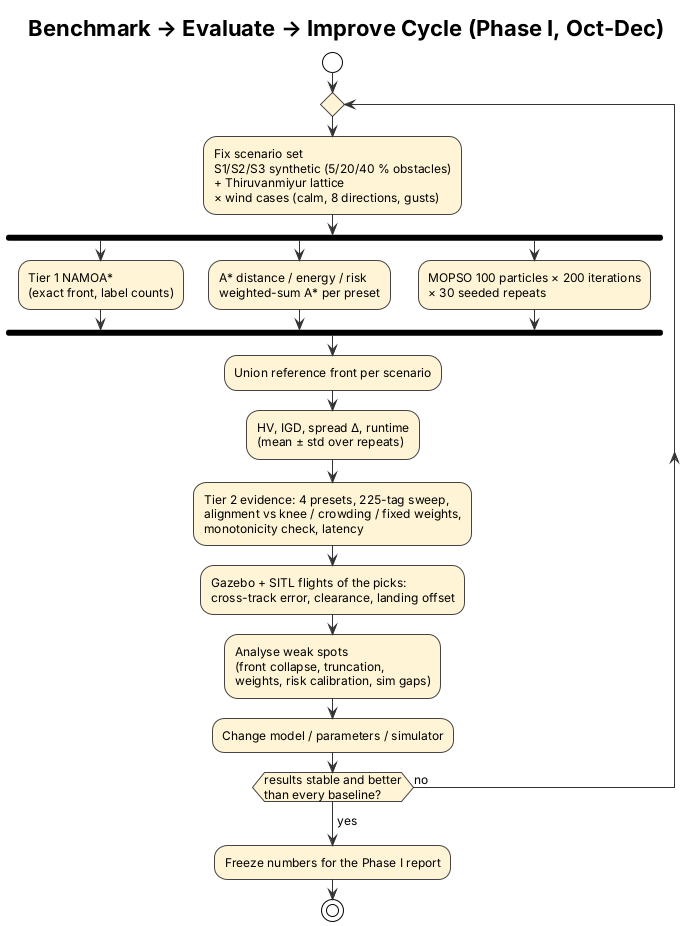
\includegraphics[width=0.62\textwidth]{eval_cycle.png}
\caption{The benchmark, evaluate and improve cycle planned for October to December}\label{fig:eval-cycle}
\end{figure}

One pass is not small. The scenario set has four graphs (the S1, S2 and S3 synthetic
scenarios plus the real-region lattice) under nine wind cases (calm and eight
compass directions), which is 36 cases. In each case we compute the exact NAMOA* front,
three single-objective A* routes, one weighted-sum A* route per payload preset, and the
MOPSO baseline \cite{r6} at the settings promised in Review~I: 100 particles,
200 iterations and 30 seeded repetitions. That is 600,000 particle updates per case,
each with a shortest-path repair, or about 21.6 million per pass. On the Tier~2 side,
each case runs all 225 tag combinations and four competing selection rules (shortest
route, knee point, NSGA-II crowding distance as in Ren et al.\ \cite{r3}, and fixed
equal weights in the style of Chokkalingam and Ganesan \cite{r1}), which is 8,100
selections per rule per pass.

A first pass has already been run on the synthetic scenarios with reduced MOPSO settings,
and it shows why more than one pass is needed. It surfaced the following problems, each of
which needs a fix and a full re-run:

\begin{enumerate}[label=(\alph*)]
  \item The obstacle density labels (5\%, 20\%, 40\%) did not reach the graph builder;
  the runner scaled the final risk instead, so the scenarios were not the ones
  described.
  \item The monotonicity check mixed scenarios and reported 660 false violations on the
  smallest run; per scenario, the count is zero.
  \item MOPSO repetitions were pooled into one archive, so there is no mean and standard
  deviation for hypervolume, IGD or spread yet.
  \item Under wind, three of the four payload presets converged on the same route on the
  benchmark graph (Section~\ref{sec:res-wind}). Whether that is the right answer or a
  side effect of min-max normalisation on a small front is an open question, and the
  answer may change Tier~2.
  \item The risk weights and battery constants are still placeholders and must be
  calibrated before any number is final.
\end{enumerate}

The margins against the baselines are also thin in places. On the 200-node scenario,
NAMOA* and MOPSO reach hypervolumes of 1.2065 and 1.2061. A gap that small needs
30 seeded repetitions and a proper statistical test before we can claim that our method
is better, and if it turns out not to be, the algorithm has to be improved and the cycle
run again. We expect several passes before the numbers are ready for the Phase~I report.

\subsection{Bringing the simulation closer to real conditions}

The simulation pipeline is built, and part of it has been tested. The mission runner has
flown planner missions on a real ArduCopter SITL build \cite{r23}: the upload and
read-back, the switch to AUTO, the landing and the disarm all worked, with a cross-track
root-mean-square error of 0.11--0.13\,m and a landing offset of at most 0.02\,m. Those
runs used ArduPilot's built-in physics, though, not the city model. The work that remains
is about fidelity:

\begin{itemize}
  \item The Gazebo world \cite{r24} has to be built from a live OpenStreetMap and DEM
  bundle and pass its gates (the world loads, the drone rests on roofs and ground
  correctly, and the real-time factor stays at or above 0.8).
  \item The Gazebo world has no wind today, while the planner now plans for wind. Until
  wind is added to the world and we verify that it actually reaches the vehicle, a
  comparison of wind cases in simulation would be meaningless.
  \item The battery model uses placeholder constants. They have to be calibrated from
  simulated flights for each payload weight class so that the feasibility filter in
  Tier~2 reflects a real F450-class airframe.
  \item Each payload preset has to be flown under several wind cases, with cross-track
  error, clearance, landing offset and end-to-end latency logged for every run.
\end{itemize}

Every mismatch between the planned and the flown route feeds back into the planner's
cost model, which brings us back to the benchmark cycle. The two loops are coupled, so
they have to run side by side.



% ============================================================
\flowchapter{Problem Statement}\label{cha:problem}

Existing UAV route planners either apply a fixed geometric selection criterion over the
Pareto front, independent of payload type (Gap~1), or fold objectives into a single
hand-tuned weighted-sum scalar before path search begins, which fixes the objective
trade-off regardless of the payload. When the payload context changes, from fragile
diagnostic samples that need vibration-minimal routing to time-critical emergency
medicine that needs shortest-path routing, an expert must re-tune the planner weights by
hand and re-run the search from scratch (Gap~2), because no algebraic mapping from
payload description to routing trade-off exists to make that re-tuning unnecessary
(Gap~3). In field conditions, that intervention is not feasible.

Formally, given:
(i)~an airspace graph $G = (V, E)$ with three-objective edge cost vectors
$\mathbf{c}(e) = [d(e),\, \varepsilon(e),\, \rho(e)]$ representing geodesic distance,
estimated energy consumption, and flight risk respectively;
(ii)~a Pareto-optimal front $\mathcal{P}$ of non-dominated routes pre-computed over $G$;
and (iii)~a payload metadata tuple $(F, W, U, P_\mathrm{lvl})$ encoding fragility class
$F \in \{1\ldots5\}$, payload weight class $W \in \{1\ldots3\}$, delivery urgency
$U \in \{1\ldots3\}$, and priority level $P_\mathrm{lvl} \in \{1\ldots5\}$, the
problem is to select the route $p^* \in \mathcal{P}$ that best satisfies the routing
requirements implied by the payload metadata, without expert re-tuning and without
re-running the multi-objective search.

The inputs are measurable quantities the operator can assign from domain knowledge (e.g.,
``this vial is fragile: $F = 5$; delivery is non-urgent: $U = 1$''). The constraints are
that selection must be deterministic, reproducible, and finish within one second of
payload tag entry. The success criterion is that the selected route's characteristics
(distance, energy, risk) match the payload's stated requirements, checked by a Tier~2
selection accuracy metric evaluated across multiple payload presets. Three conditions
follow from the gaps. The selected route $p^*$ must depend on $(F, W, U, P_\mathrm{lvl})$,
not on front geometry alone (Gap~1). The front $\mathcal{P}$ must be reused across
missions between scheduled refreshes instead of rebuilt each time (Gap~2). The map from
$(F, W, U, P_\mathrm{lvl})$ to $p^*$ must be an explicit algebraic formula, not an
expert-set rule or a lookup table (Gap~3).

\section{Weather Dependence of the Problem}

The edge costs are functions of the weather. Writing $\omega$ for a
weather snapshot (wind speed, wind direction, gust, rain, visibility), the cost of an
edge is $\mathbf{c}(e;\omega) = [d(e),\, \varepsilon(e;\omega),\, \rho(e;\omega)]$ and the
front is $\mathcal{P}(\omega)$. Distance stays fixed, but energy and risk depend on how
the wind meets each edge. This does not change the selection problem itself. It does mean
that a stored front is only valid while $\omega$ stays close to the snapshot it was built
for, which is why the front is refreshed on a schedule and on weather drift. If $\omega$
breaches the go/no-go limits, no route is selected at all and the mission is held.

\section{Inputs, Outputs and Success Criteria}

Table~\ref{tab:ps-io} lists what the system takes in, what it returns, and how each part
of the problem is judged.

\begin{table}[H]
\centering\caption{Inputs, outputs, constraints and success criteria}\label{tab:ps-io}\small
\begin{tabularx}{\textwidth}{L{3.0cm} Y}
\toprule
\textbf{Item} & \textbf{Definition}\\
\midrule
Region input & Centre point and box size; terrain (DEM), OSM buildings, restricted zones, water and land use for that box\\
Weather input & Snapshot $\omega$ from Open-Meteo (wind at 80\,m, gust, rain, visibility, WMO code)\\
Mission input & Depot, destination and payload tuple $(F, W, U, P_\mathrm{lvl})$\\
Tier~1 output & Stored Pareto front $\mathcal{P}(\omega)$ with graph hash, weather snapshot and expiry\\
Tier~2 output & Selected route $p^*$ with waypoints (lat, lon, altitude), weights, ranks and point type, or a HOLD advisory\\
Mission output & QGC WPL~110 \texttt{.waypoints} and QGroundControl \texttt{.plan} files\\
Hard constraints & Cruise at least 60\,m above ground and 15\,m above roofs; at most 120\,m above ground; no entry into restricted zones; route energy within 80\% of battery capacity\\
Tier~1 criteria & Hypervolume and IGD at least as good as every baseline on each scenario; no dominated or duplicate routes in the front\\
Tier~2 criteria & Selection under 1\,s; zero monotonicity violations over all 225 tag combinations; non-extreme picks for mixed payloads\\
Simulation criteria & Cross-track error, clearance margin and landing offset of the flown route in Gazebo and SITL\\
\bottomrule
\end{tabularx}
\end{table}


% ============================================================
\flowchapter{Methodology}\label{cha:methodology}

The system rests on one design decision: separate Pareto front construction (Tier~1)
from route selection (Tier~2), for the reasons in Chapter~\ref{cha:problem}. The
front is built once per delivery region and refreshed periodically, not per mission. A
mission that arrives between refreshes runs only Tier~2, which reads the payload tag and
returns a route from the current front in a fraction of a second.

The system follows one workflow. Environment data for a delivery region
is collected and cached. The airspace graph is built from it, with node and edge
selection and a shared cost pipeline. Tier~1 computes the Pareto front and stores it.
Tier~2 turns each payload tag into a route, and the route is exported as a mission and
flown in simulation. Baseline planners and an evaluation module score every stage, and
their findings flow back into the model. Figure~\ref{fig:methodology} gives an overview
of this workflow.

\begin{figure}[H]
\centering

\includegraphics[width=\textwidth]{methodology.png}
\caption[Methodology overview: Two-Tier Payload-Aware UAV Route Planning]{Methodology
overview: Tier~1 Pareto front construction feeding Tier~2 payload-aware route
selection, with mission output, UAV control and performance evaluation.}\label{fig:methodology}
\end{figure}

\section{Architectural Design for Proposed System}

Figure~\ref{fig:architecture} shows the system architecture. It has five layers. The
environment data layer fetches weather, terrain and OpenStreetMap layers and caches them
on disk, so that a network failure falls back to the last good copy instead of stopping
the planner. Module~1 turns these layers into a directed airspace graph whose edges carry
a three-objective cost vector. Tier~1 (Module~2) computes the Pareto front over that graph
and keeps it in a front store with the metadata needed to decide when it is stale. Tier~2
(Module~4) reads the operator's payload tags and returns one route from the stored front,
or a HOLD advisory when the weather or the battery rules the mission out. The output layer
(Modules~6 and~7) writes the mission file and flies it in Gazebo with ArduPilot SITL.
Modules~3 and~5 sit beside the main path: they run the baseline planners and compute the
quality metrics used in Chapter~\ref{cha:results}.

\begin{figure}[H]
\centering
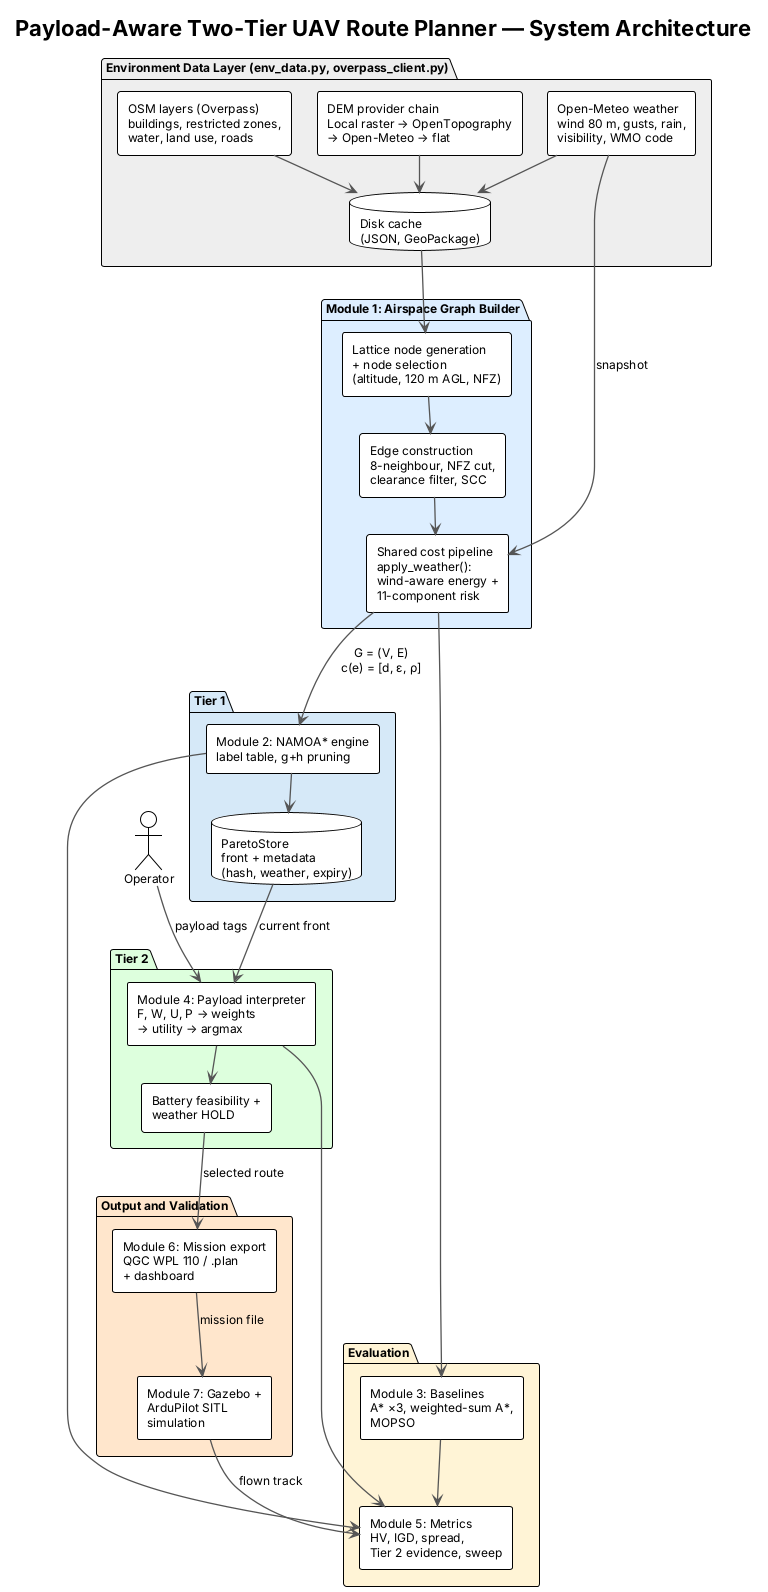
\includegraphics[width=0.66\textwidth]{arch.png}
\caption[System architecture]{System architecture. Tier~1 builds
and stores the front per region and weather window; Tier~2 selects a route per payload
tag; Modules~6 and~7 export and fly it.}\label{fig:architecture}
\end{figure}

Every edge $e = (u, v)$ of the airspace graph carries the cost vector
\[
  \mathbf{c}(e;\omega) = \bigl[d(e),\; \varepsilon(e;\omega),\; \rho(e;\omega)\bigr]
\]
where $d(e)$ is the three-dimensional flight distance of the segment in kilometres,
$\varepsilon(e;\omega)$ is the wind- and grade-aware energy proxy, and
$\rho(e;\omega)$ is the cumulative risk exposure along the segment under weather
snapshot $\omega$. Section~\ref{sec:m1} defines all three.

The three optimisation objectives are: (1)~minimise route distance $d$; (2)~minimise
energy consumption $\varepsilon$; and (3)~minimise flight risk $\rho$. A route $p$
dominates route $q$ if $p$ is at least as good as $q$ on all three objectives and
strictly better on at least one. The Pareto front $\mathcal{P}$ is the set of all
non-dominated routes.

Figure~\ref{fig:sequence} follows a single mission through the system, from the moment
the operator enters the payload tags to the moment the drone lands.

\begin{figure}[H]
\centering
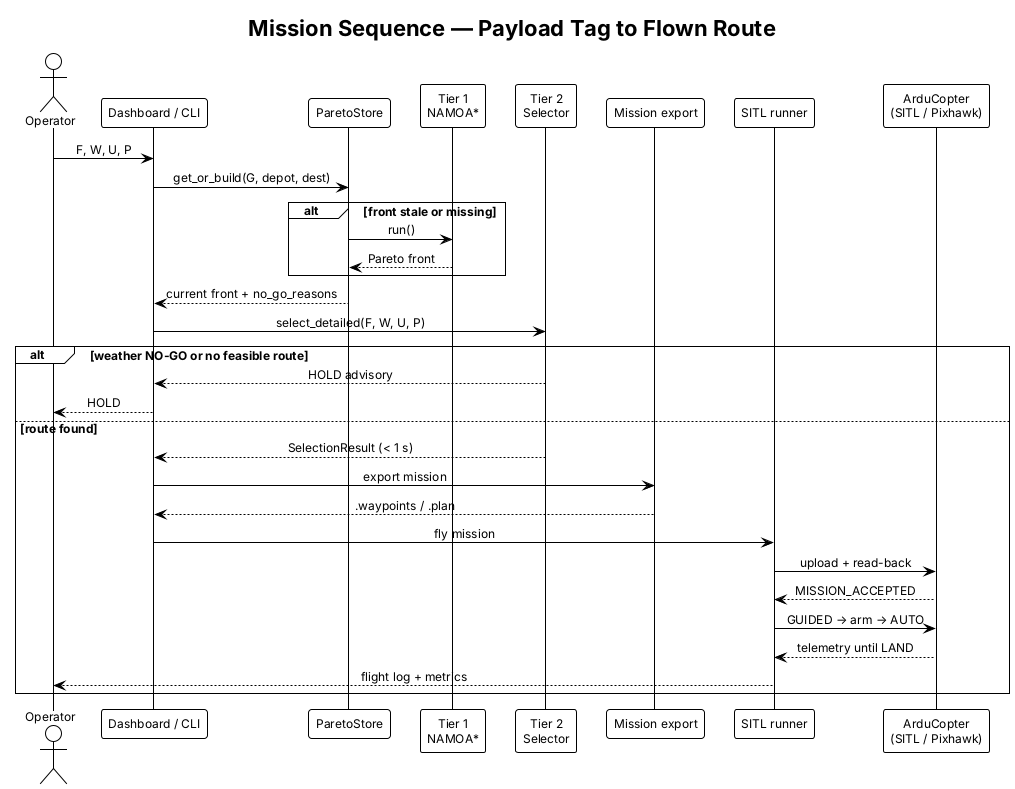
\includegraphics[width=0.95\textwidth]{mission_sequence.png}
\caption{Mission sequence from payload tag entry to the flown route}\label{fig:sequence}
\end{figure}

\section{Modules}

The code is organised into seven modules. The numbering follows the source files, so
Module~3 holds the baselines and Module~4 holds Tier~2. Each module is described below in
terms of its purpose, inputs, processing, outputs and dependencies.

% ------------------------------------------------------------
\subsection{Module 1: Airspace Graph Builder}\label{sec:m1}

\subsubsection{Purpose, inputs and outputs}

Module~1 builds the delivery airspace graph $G = (V, E)$. Its inputs are the region
(centre, box size and lattice spacing), the environment layers described next, and a
weather snapshot $\omega$. Its output is a directed NetworkX graph whose nodes carry
position and altitude and whose edges carry the static features, the per-component risk
breakdown, and the cost vector $[d, \varepsilon, \rho]$. The global weather go/no-go state
is stored on the graph itself so that Tier~2 can read it. Two builders share the same cost
pipeline: a lattice builder over a real region and a seeded
synthetic builder used for controlled benchmarks. Figure~\ref{fig:m1-pipeline} gives the
whole pipeline.

\begin{figure}[H]
\centering
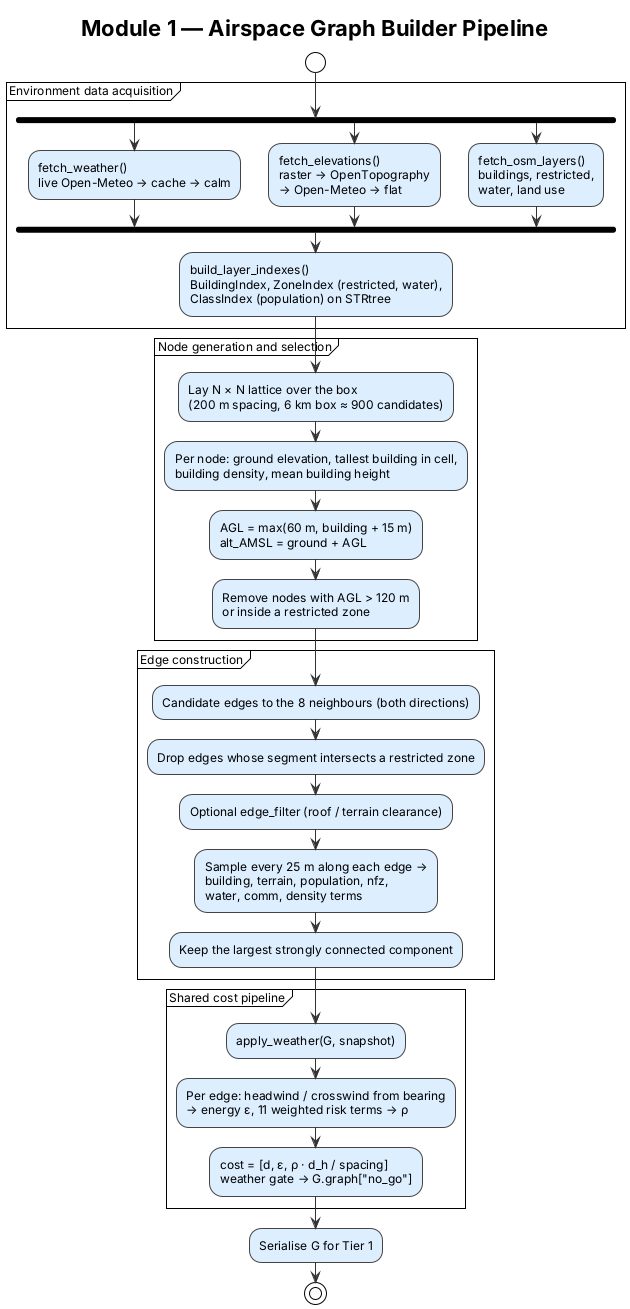
\includegraphics[width=0.62\textwidth]{module1_pipeline.png}
\caption{Module~1 pipeline: data acquisition, node selection, edge construction and the
shared cost pipeline}\label{fig:m1-pipeline}
\end{figure}

\subsubsection{Environment data acquisition}

Weather comes from the Open-Meteo forecast API \cite{r20}, which needs no key. The module
reads the current 10\,m wind, gust, precipitation, visibility and WMO weather code, and
the hourly 80\,m wind speed and direction. The hourly row is chosen by matching the
response's own local time string, so no time-zone conversion is involved. Results are cached; with no network the last cached snapshot is used, and with no
cache the planner assumes calm air so that runs stay deterministic.

Terrain comes from an elevation provider chain tried in order: a local GeoTIFF if one is
configured, the OpenTopography Copernicus 30\,m service (with an API key), the Open-Meteo
elevation service (Copernicus 90\,m, batches of 100 points), and finally flat ground with
a warning. Every value is cached under a key rounded to about one metre.

OpenStreetMap layers are fetched through a multi-endpoint Overpass client with retries, a
busy-wait cap and an identifying user agent. Four layers are extracted: building
footprints, restricted zones, water bodies (including a sea polygon built from the
coastline) and land use with points of interest and major roads. They are cached as
GeoPackage files and indexed in local metric coordinates with Shapely STRtree structures:
a building index (heights, cell maxima, density, mean height), a zone index for
restricted areas and another for water (containment, distance, segment intersection), and
a class index for population exposure.

\subsubsection{Lattice generation and node selection}

The region is covered by an $n \times n$ lattice in a local equirectangular frame
centred on the region, with $n = \mathrm{round}(\mathit{box}/\mathit{spacing})$. The
default 6\,km box at 200\,m spacing gives 900 candidate nodes. Each candidate is then put
through the selection rule of Figure~\ref{fig:node-select}. For node $k$ with ground
elevation $z_k$ and tallest building $b_k$ in its cell,
\begin{equation}
  \mathrm{AGL}_k = \max\bigl(H_\mathrm{cruise},\; b_k + C\bigr), \qquad
  \mathrm{alt}_k = z_k + \mathrm{AGL}_k \label{eq:alt}
\end{equation}
with $H_\mathrm{cruise} = 60$\,m and clearance $C = 15$\,m. A node with
$\mathrm{AGL}_k > 120$\,m is blocked, because it cannot be flown legally under the Drone
Rules, 2021 \cite{r21}. A node inside a restricted polygon is removed. Every surviving
node stores its position in both frames, its ground elevation, the building height,
density and mean height of its cell, its height above ground and its altitude above mean
sea level.

\begin{figure}[H]
\centering
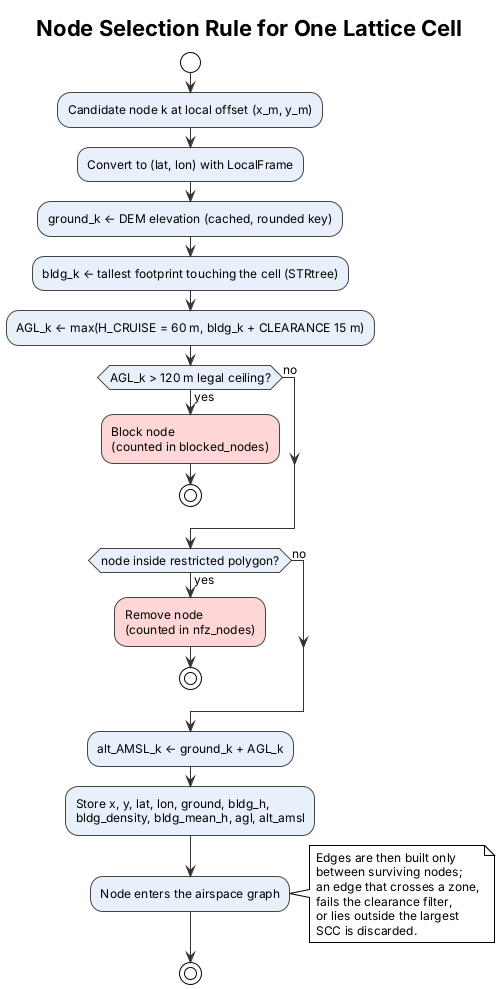
\includegraphics[width=0.55\textwidth]{node_selection.png}
\caption{Selection rule applied to each candidate lattice node}\label{fig:node-select}
\end{figure}

\subsubsection{Edge construction and pruning}

Each surviving node is linked to its eight neighbours in both directions, so the graph is
directed from the start. Three filters then remove edges. The first drops any edge whose
straight segment intersects a restricted polygon, which stops a route from clipping the
corner of a zone between two legal nodes. The second is an optional hook,
\texttt{edge\_filter}, that the simulation module uses for hard roof and terrain clearance.
The third keeps only the largest strongly connected component, so that every remaining
node can reach every other.

For each kept edge the horizontal haversine length $d_h$, the forward-azimuth bearing
$\theta$, the grade $g = \Delta\mathrm{alt}/d_h$ and the three-dimensional length
$d = \sqrt{d_h^2 + \Delta\mathrm{alt}^2}$ are stored. The bearing uses
\begin{equation}
  \theta = \operatorname{atan2}\bigl(\sin\Delta\lambda\cos\varphi_2,\;
  \cos\varphi_1\sin\varphi_2 - \sin\varphi_1\cos\varphi_2\cos\Delta\lambda\bigr)
\end{equation}
so that the east component is scaled by $\cos\varphi$.

\subsubsection{Static risk terms}

Static terms do not depend on the weather. They are computed once per build by sampling
each edge every 25\,m and flying the straight line between the two endpoint altitudes.
At each sample $k$ the module knows the flight altitude, the ground height, the tallest
roof directly below and the tallest roof within 30\,m. Table~\ref{tab:risk} lists all
eleven components, both static and weather-dependent, with the weight each one carries in
the edge score
\begin{equation}
  \rho_\mathrm{edge} = \operatorname{clip}\Bigl(\sum_k w_k\,\rho_k,\; 0,\; 1\Bigr), \qquad
  \rho(e;\omega) = \rho_\mathrm{edge}\cdot\frac{d_h}{s} \label{eq:risk}
\end{equation}
where $s$ is the lattice spacing. Multiplying by $d_h/s$ turns the per-edge score into a
cumulative exposure, so a diagonal hop counts $\sqrt{2}$ times an axis hop and the risk of
a route grows with the distance flown through risky air.

\small
\begin{xltabular}{\textwidth}{L{2.4cm} Y L{1.0cm}}
\caption{Risk components (every $\rho_k \in [0,1]$) and their weights}\label{tab:risk}\\
\toprule
\textbf{Component} & \textbf{Model} & $\boldsymbol{w_k}$\\
\midrule
\endfirsthead
\multicolumn{3}{l}{\small\itshape Table \thetable\ (continued)}\\
\toprule
\textbf{Component} & \textbf{Model} & $\boldsymbol{w_k}$\\
\midrule
\endhead
\bottomrule
\endlastfoot
Obstacle & Seeded obstacle discs, $0.9(1 - r/R)$ inside a disc (synthetic graphs only) & 1.00\\
Building & Mean over samples of $[\text{roof within 30\,m}]\cdot\bigl(1-\operatorname{clip}(m/60)\bigr)$, $m$ = margin above that roof & 0.60\\
Terrain & $\max\bigl(1-\operatorname{clip}(m_{\min}/15),\ \operatorname{clip}(\lvert g\rvert/0.30)\bigr)$: lowest clearance margin or sudden altitude change & 0.30\\
Wind & $\operatorname{clip}(C\!W/40)$, crosswind against a 40\,km/h saturation speed & 0.30\\
Gust & $\operatorname{clip}\bigl(0.5\max(0, \mathit{gust} - v)/40\bigr)$ & 0.30\\
Weather & $0.5\operatorname{clip}(\mathit{rain}/7.5) + 0.5\operatorname{clip}(1 - \mathit{vis}/10\,\mathrm{km})$, uniform over the graph & 0.20\\
Population & Mean land-use class score along the edge (our values, ranked in the spirit of SORA \cite{r22}): assembly 1.0, commercial 0.7, major road 0.6, residential 0.5, industrial 0.3 & 0.50\\
No-fly buffer & $\max_k \exp(-\delta_k/150\,\mathrm{m})$ to the nearest restricted zone, zero beyond 600\,m & 0.80\\
Water & Fraction of samples over water (risk of payload loss) & 0.30\\
Comm/GPS & $\operatorname{clip}(\mathit{density}/0.30)\cdot\operatorname{clip}(\bar{h}/30\,\mathrm{m})$, urban canyon & 0.20\\
Turbulence & $\operatorname{clip}(\mathit{density}/0.30)\cdot\operatorname{clip}(v/40)$ & 0.20\\
\end{xltabular}
\normalsize

The weights are design values chosen to put restricted zones, buildings and crowds ahead
of weather terms. They have not been calibrated against flight data yet, and calibrating
them is part of the evaluation cycle.

\subsubsection{Wind-aware energy model}

For an edge on bearing $\theta_\mathrm{edge}$ and a wind of speed $v$ blowing from
$\theta_\mathrm{from}$ (the meteorological convention), the headwind and crosswind are
\begin{equation}
  H\!W = v\cos(\theta_\mathrm{edge} - \theta_\mathrm{from}), \qquad
  C\!W = v\,\lvert\sin(\theta_\mathrm{edge} - \theta_\mathrm{from})\rvert \label{eq:hwcw}
\end{equation}
A positive $H\!W$ is a headwind. The energy proxy of the edge is
\begin{equation}
  \varepsilon = d\left(1 + \lvert g\rvert + \beta_h\frac{\max(0, H\!W)}{V_c}
  + \beta_c\frac{C\!W}{V_c}\right) \label{eq:energy}
\end{equation}
with cruise airspeed $V_c = 36$\,km/h, $\beta_h = 0.40$ and $\beta_c = 0.15$. A tailwind is
clamped to zero benefit. This is a deliberate choice: it keeps $\varepsilon \geq d$ on
every edge, which the Tier~1 heuristic relies on. The wind speed itself is the 80\,m
forecast when available, otherwise the 10\,m value lifted to cruise height with the
power law $v_h = v_{10}(h/10)^{0.25}$ \cite{r19}. A gust factor measured at 10\,m is
applied to the wind at flight height. Figure~\ref{fig:wind} shows the per-edge
computation.

\begin{figure}[H]
\centering
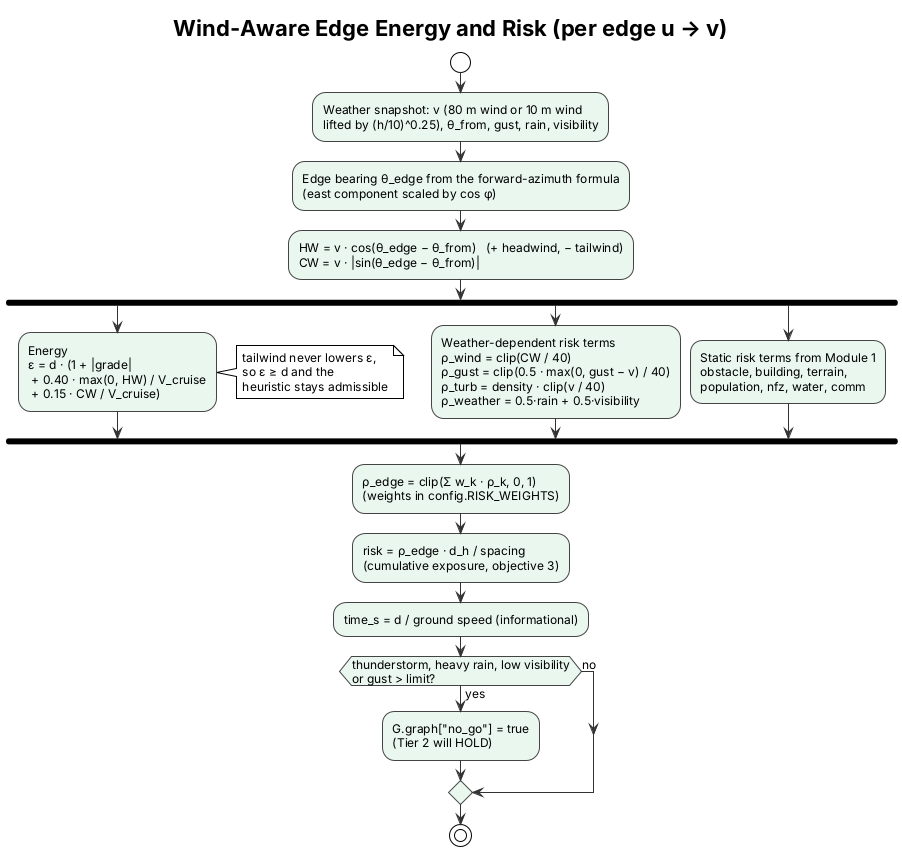
\includegraphics[width=0.78\textwidth]{wind_model.png}
\caption{Per-edge wind decomposition into energy and risk}\label{fig:wind}
\end{figure}

\subsubsection{Weather-dependent risk and the go/no-go gate}

Four of the eleven risk components change with the weather: crosswind, gust excess,
turbulence and the uniform rain and visibility term (Table~\ref{tab:risk}). Because
crosswind depends on the edge heading, the same wind makes some corridors riskier than
others, and a change of direction alone can move the low-risk end of the front to a
different part of the map. The function \texttt{apply\_weather(G, $\omega$)} recomputes
energy, risk, the component breakdown and an informational flight time on every edge from
the stored static features. It is idempotent, so the same graph can be re-costed for a new
snapshot without rebuilding any spatial layer.

The weather gate sits on top of this. The mission is a no-go when the WMO code reports a
thunderstorm (95--99), when rain reaches 7.5\,mm/h, when visibility falls below 1\,km, or
when gusts exceed 45\,km/h, a provisional limit for an F450-class airframe. The reasons
are written to the graph and Tier~2 refuses to select a route while any reason is present.

\subsubsection{Synthetic scenario builder}

Benchmarks need graphs whose difficulty we control. The synthetic builder places nodes on
a jittered grid of about 1.3\,km spacing with 8-neighbour edges, generates a terrain field
from a few seeded Gaussian hills, and drops obstacle discs until a target fraction of the
area is covered, with half of them placed along the source-to-target diagonal so that the
shortest route has to cross risk. The wind is seeded too (12--28\,km/h with a gust factor
of 1.4). Every random draw comes from a seed-derived generator, so a scenario is
reproduced exactly from its seed. The same \texttt{apply\_weather} pipeline costs the
synthetic edges, which keeps benchmark and real-region results comparable.

% ------------------------------------------------------------
\subsection{Module 2: Tier 1 Pareto Front Engine (NAMOA*)}\label{sec:m2}

\subsubsection{Purpose, inputs and outputs}

Module~2 computes the exact set of non-dominated routes between a source and a target.
Its inputs are the costed graph from Module~1, the two end nodes and an expansion cap. Its
output is the Pareto front $\mathcal{P}$, a list of cost vectors and node paths, together
with diagnostics: whether the search was truncated by the cap, how many labels were
expanded and generated, and the runtime.

\subsubsection{Labels and dominance}

The engine follows NAMOA* \cite{r17}. Every partial path is a label
$(\mathit{node}, \mathbf{g}, \mathit{parent})$ held in a flat table, and a path is rebuilt
at the end by walking parent ids. Nothing is copied when a label is pushed, which matters
once the label count runs into thousands. A new label $\mathbf{g}'$ at node $v$ is
discarded if any existing label at $v$ weakly dominates it ($\leq$ in every objective
within a small tolerance). Equal vectors count as dominated, so the front never contains
duplicates. Labels that the new one dominates are marked dead and skipped when popped.
No visited set is needed: every edge has positive distance, so a path that revisits a node
is dominated by its own earlier label at that node, and cycles die in the dominance check.

\subsubsection{Admissible vector heuristic and pruning}

The heuristic for node $v$ is $\mathbf{h}(v) = [h, h, 0]$, where $h$ is the great-circle
distance from $v$ to the target. It is admissible for all three objectives. For distance,
every edge satisfies $d \geq d_h$, and the horizontal lengths of any path to the target sum
to at least $h$. For energy, Equation~(\ref{eq:energy}) gives $\varepsilon \geq d$, so the
same bound holds. For risk, $\rho \geq 0$. A label is pruned when the current front weakly
dominates $\mathbf{g} + \mathbf{h}$, both when it is generated and again when it is popped,
because the front may have improved in between. The open list is ordered by
$\lVert\mathbf{g} + \mathbf{h}\rVert$, which tends to complete good routes early and so
tightens the pruning sooner.

\subsubsection{Truncation and front thinning}

The expansion cap protects the planner from a runaway search on a dense graph. When the
cap is hit, the engine checks whether any live label could still improve the front after
adding its heuristic. Only then is the result flagged as truncated, and a warning is
printed. For large fronts an optional $\varepsilon$-dominance thinning step can cap the
front at $N$ routes. Objectives are min-max normalised and cut into $\varepsilon$-boxes,
one route survives per non-dominated box, $\varepsilon$ is found by bisection, and the three
single-objective extremes are always kept because Tier~2 normalises against them. Thinning
is off by default so that benchmarks use the exact front.

\begin{algorithm}[H]
\caption{NAMOA* with a label table (Tier~1)}\label{alg:tier1}
\begin{algorithmic}[1]
\Require Directed graph $G=(V,E)$, source $s$, target $t$, costs $\mathbf{c}(u,v)=[d,\varepsilon,\rho]$, cap $M$
\Ensure Pareto front $\mathcal{P}$, flag $\mathit{truncated}$
\State $L \gets [(s, [0,0,0], -1)]$; \quad $\mathit{at}[s] \gets \{0\}$; \quad $F \gets \emptyset$; \quad $\mathit{Open} \gets \{(\lVert\mathbf{h}(s)\rVert, 0)\}$
\While{$\mathit{Open} \neq \emptyset$}
  \If{$\mathit{expanded} \geq M$}
    \State $\mathit{truncated} \gets \exists$ live $\ell \in \mathit{Open}$ with $F \not\preceq \mathbf{g}_\ell + \mathbf{h}(u_\ell)$; \textbf{break}
  \EndIf
  \State $\ell = (u, \mathbf{g}) \gets$ \Call{PopMin}{$\mathit{Open}$}
  \If{$\ell$ is dead \textbf{or} $F \preceq \mathbf{g} + \mathbf{h}(u)$} \textbf{continue} \EndIf
  \State $\mathit{expanded} \gets \mathit{expanded} + 1$
  \For{each successor $v$ of $u$}
    \State $\mathbf{g}' \gets \mathbf{g} + \mathbf{c}(u,v)$
    \If{$\exists\, o \in \mathit{at}[v] : \mathbf{g}_o \preceq \mathbf{g}'$} \textbf{continue} \Comment{node-level dominance}
    \EndIf
    \If{$F \preceq \mathbf{g}' + \mathbf{h}(v)$} \textbf{continue} \Comment{front pruning on $g+h$}
    \EndIf
    \State mark dead every $o \in \mathit{at}[v]$ with $\mathbf{g}' \preceq \mathbf{g}_o$
    \State append label $(v, \mathbf{g}', \ell)$ to $L$ and to $\mathit{at}[v]$
    \If{$v = t$}
      \State $F \gets \{f \in F : \mathbf{g}' \not\preceq f\} \cup \{\mathbf{g}'\}$
    \Else
      \State push $(\lVert\mathbf{g}' + \mathbf{h}(v)\rVert, \text{label})$ onto $\mathit{Open}$
    \EndIf
  \EndFor
\EndWhile
\State rebuild each route in $F$ by following parent ids; \Return $\mathcal{P}$, $\mathit{truncated}$
\end{algorithmic}
\end{algorithm}

Here $\preceq$ is weak dominance. Figure~\ref{fig:tier1} gives the same procedure as an
activity diagram.

\begin{figure}[H]
\centering
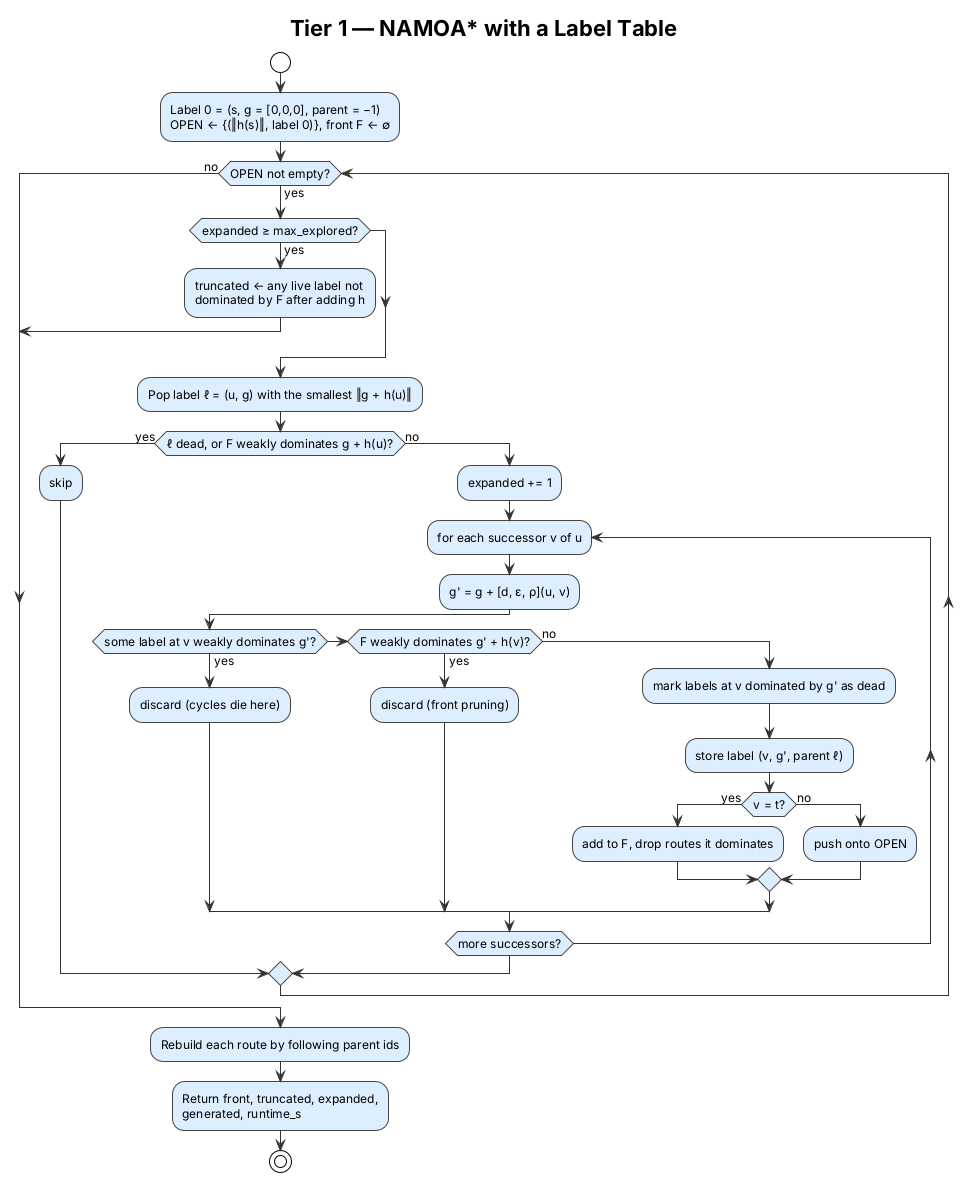
\includegraphics[width=0.68\textwidth]{tier1.png}
\caption{Tier~1 activity flow: NAMOA* with a label table}\label{fig:tier1}
\end{figure}

\subsubsection{Pareto front store and refresh}

The front is built per region and reused, so the system needs a rule for when reuse is
safe. The front store saves one JSON record per (region, source, target). Each record
holds the front, a SHA-256 hash over the node ids and static edge attributes (never the
weather-dependent costs, so a change of weather alone does not alter the hash), the
weather snapshot it was built for, the creation time, a validity limit three hours later,
the truncation flag and the search diagnostics. An optional identity field ties the front
to a simulation bundle.

On each request the store lists the reasons the record cannot be reused
(Figure~\ref{fig:store}): no record, a forced refresh, a different static graph, a
different identity, expiry, or weather drift. Drift means the wind speed has moved by more
than 10\,km/h, the direction has turned by more than 45$^\circ$ while the wind is above
10\,km/h, the gust has moved by more than 15\,km/h, or the go/no-go state has flipped. If
there is no reason, Tier~2 runs against the stored front and no search happens. If there
is one, only \texttt{apply\_weather} and Tier~1 run again; the spatial layers stay cached.
A helper also builds one front per delivery point for a depot, snapping each point's
latitude and longitude to the nearest lattice node.

\begin{figure}[H]
\centering
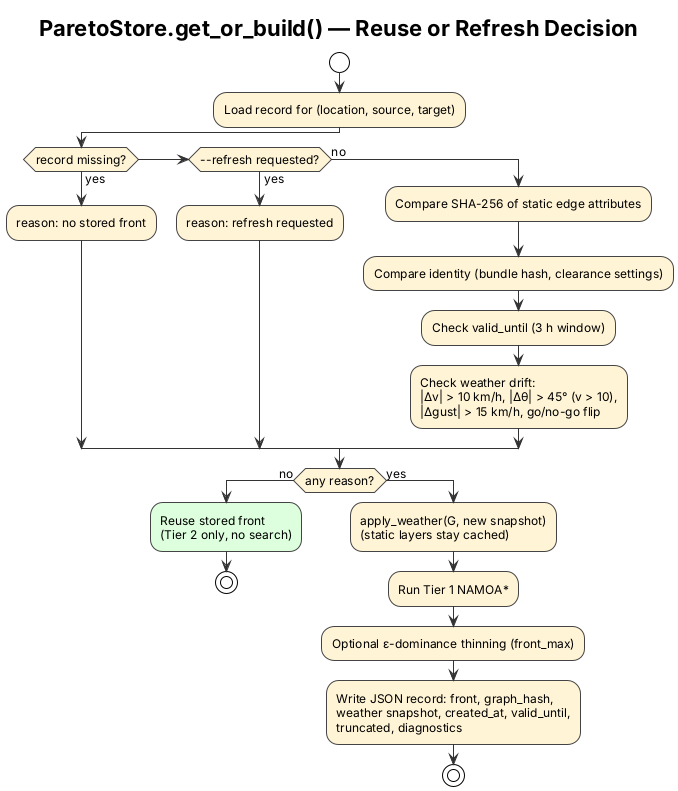
\includegraphics[width=0.58\textwidth]{store.png}
\caption{Front store decision: reuse the stored front or rebuild it}\label{fig:store}
\end{figure}

% ------------------------------------------------------------
\subsection{Module 3: Baseline Planners}\label{sec:m3}

\subsubsection{Purpose}

Module~3 holds the planners that Tier~1 and Tier~2 are compared against. They read the
same costed graph, so any difference in the results comes from the search method and not
from the data.

\subsubsection{Single-objective A*}

Three A* searches minimise distance, energy and risk separately. The distance search
uses the haversine distance to the target as its heuristic, which is admissible for the
same reason as in Tier~1. The energy and risk searches use a zero heuristic, which makes
them Dijkstra searches behind the same interface. Each returns one route, the extreme
point of the front for its objective. Their purpose in the comparison is to show what a
planner that ignores the trade-off would fly.

\subsubsection{Weighted-sum A*}

The weighted-sum baseline scalarises the cost vector with the Tier~2 weights of a payload
preset, $\sum_j w_j c_j(e)/s_j$, where each scale $s_j$ is the spread of objective $j$
across the three single-objective routes, and runs A* on that scalar. This is the classic approach that the problem
statement criticises. It can only reach supported points of the front (points on its
convex hull), so comparing it with Tier~2 shows whether scoring the full front reaches
routes that a single scalarised search cannot.

\subsubsection{MOPSO}

The population-based baseline adapts multi-objective particle swarm optimisation
\cite{r6} to graph routes. A particle is a valid source-to-target path. The swarm is
seeded with the three single-objective routes, an equal-weight route and biased random
walks. In each iteration a particle samples a random preference vector, follows its
personal best or a leader drawn from the archive for part of the way, and is repaired to
the target with a weighted shortest suffix. Only valid non-dominated paths enter an
archive of bounded size. The settings for the reported experiments are 100 particles,
200 iterations, an archive of 100 and 30 seeded repetitions; a smaller smoke setting is
used for quick checks.

% ------------------------------------------------------------
\subsection{Module 4: Tier 2 Payload Metadata Interpreter}\label{sec:m4}

\subsubsection{Purpose, inputs and outputs}

Module~4 turns the payload description into a route. Its inputs are the stored front, the
weather go/no-go reasons from the graph, and the four tags $(F, W, U, P_\mathrm{lvl})$. Its
output is a selection record: the tags, the derived weights, the selected route index,
cost vector and waypoints with latitude, longitude and altitude, the normalised scores,
the selected route's rank on each objective, whether it is an extreme or non-extreme
point, the latency, the number of battery-feasible routes and, when no route can be
flown, a HOLD advisory. The record is written to JSON and CSV.

\subsubsection{Tag validation}

Each tag must be an integer in its range: $F \in \{1..5\}$, $W \in \{1..3\}$,
$U \in \{1..3\}$, $P_\mathrm{lvl} \in \{1..5\}$. Booleans and floats are rejected. A bad
tag raises an error before any weight is derived, so a typing mistake at the ground
station cannot quietly change the route.

\subsubsection{The algebraic bridge}

The Tier~2 algebraic bridge maps each of the four payload metadata tags to exactly one
Tier~1 routing objective, as shown in Table~\ref{tab:semantic-mapping}.

\begin{table}[H]
\centering\caption{Semantic mapping: payload metadata tags to Tier~1 routing objectives}\label{tab:semantic-mapping}\small
\begin{tabularx}{\textwidth}{L{2.8cm} L{1.4cm} Y L{4.2cm}}
\toprule
\textbf{Payload Tag} & \textbf{Range} & \textbf{Maps to Tier~1 Objective} & \textbf{Reasoning}\\
\midrule
Fragility class $F$      & 1--5 & $w_\mathrm{risk}$ (flight risk weight)   & Fragile items need low-vibration, low-risk corridors\\
Payload weight class $W$ & 1--3 & $w_\mathrm{energy}$ (energy weight)  & Heavier payload increases hover/lift power draw $\Rightarrow$ higher energy cost\\
Delivery urgency $U$     & 1--3 & $w_\mathrm{dist}$ (distance weight)       & Time-critical deliveries need the shortest path\\
Priority level $P_\mathrm{lvl}$ & 1--5 & Tie-breaker amplifier           & Scales the dominant weight when scores are close\\
\bottomrule
\end{tabularx}
\end{table}

From the payload tags, three routing objective weights are derived algorithmically with
no expert input:
\begin{align}
  r_\mathrm{raw} &= F \times 2, \quad d_\mathrm{raw} = U \times 3, \quad e_\mathrm{raw} = W \times 2 \label{eq:raw}\\
  w_\mathrm{risk} &= \frac{r_\mathrm{raw}}{r_\mathrm{raw} + d_\mathrm{raw} + e_\mathrm{raw}}, \quad
  w_\mathrm{dist} = \frac{d_\mathrm{raw}}{r_\mathrm{raw} + d_\mathrm{raw} + e_\mathrm{raw}}, \quad
  w_\mathrm{energy} = \frac{e_\mathrm{raw}}{r_\mathrm{raw} + d_\mathrm{raw} + e_\mathrm{raw}} \label{eq:weights}
\end{align}
The multipliers (2 for fragility and payload weight, 3 for urgency) encode the
assumption that urgency is more penalty-sensitive than fragility or payload weight in the
UAV medical delivery context. Payload weight is tied to the energy objective because a
heavier payload directly increases hover and lift power draw; no such direct physical
link holds for risk or distance.

For each Pareto point $p_i$ with objective values $(d_i, \varepsilon_i, \rho_i)$,
min-max normalised values $\tilde{d}_i$, $\tilde{\varepsilon}_i$, $\tilde{\rho}_i$ are
computed over the full Pareto front $\mathcal{P}$. The utility score is:
\begin{equation}
  \mathrm{score}(p_i) = w_\mathrm{dist}\cdot(1 - \tilde{d}_i) + w_\mathrm{energy}\cdot(1 - \tilde{\varepsilon}_i) + w_\mathrm{risk}\cdot(1 - \tilde{\rho}_i) \label{eq:score}
\end{equation}
The selected mission route is $p^* = \arg\max_{p_i \in \mathcal{P}}\,\mathrm{score}(p_i)$.
For high-priority missions ($P_\mathrm{lvl} \geq 4$), the dominant weight is amplified
by $0.1 \times w_\mathrm{max}$ to sharpen the selection.

Table~\ref{tab:presets} gives the weights that the bridge produces for the four reference
presets. Only emergency medicine has $P_\mathrm{lvl} \geq 4$, so it is the only preset
whose dominant weight is amplified.

\begin{table}[H]
\centering\caption{Reference payload presets and their derived weights}\label{tab:presets}\small
\begin{tabular}{l c c c c c c c}
\toprule
\textbf{Preset} & $F$ & $W$ & $U$ & $P_\mathrm{lvl}$ & $w_\mathrm{risk}$ & $w_\mathrm{dist}$ & $w_\mathrm{energy}$\\
\midrule
Fragile medical sample & 5 & 1 & 1 & 3 & 0.667 & 0.200 & 0.133\\
Emergency medicine     & 1 & 1 & 3 & 5 & 0.144 & 0.712 & 0.144\\
Disaster relief        & 1 & 3 & 1 & 2 & 0.182 & 0.273 & 0.545\\
Mixed cargo            & 3 & 2 & 2 & 3 & 0.375 & 0.375 & 0.250\\
\bottomrule
\end{tabular}
\end{table}

\begin{algorithm}[H]
\caption{Payload-Driven Pareto Route Selection (Tier~2)}\label{alg:tier2}
\begin{algorithmic}[1]
\Require Pareto front $\mathcal{P} = \{(d_i,\varepsilon_i,\rho_i)\}$, payload tags $F, W, U, P_\mathrm{lvl}$
\Ensure Selected mission route $p^*$
\State $r_\mathrm{raw} \gets F \times 2$; \quad $d_\mathrm{raw} \gets U \times 3$; \quad $e_\mathrm{raw} \gets W \times 2$
\State $\mathit{total} \gets r_\mathrm{raw} + d_\mathrm{raw} + e_\mathrm{raw}$
\State $w_\mathrm{risk} \gets r_\mathrm{raw}/\mathit{total}$; \quad $w_\mathrm{dist} \gets d_\mathrm{raw}/\mathit{total}$; \quad $w_\mathrm{energy} \gets e_\mathrm{raw}/\mathit{total}$
\If{$P_\mathrm{lvl} \geq 4$} \Comment{high-priority amplification}
    \State $w_\mathrm{max} \gets \max(w_\mathrm{risk}, w_\mathrm{dist}, w_\mathrm{energy})$
    \State add $0.1 \times w_\mathrm{max}$ to whichever of $w_\mathrm{risk}, w_\mathrm{dist}, w_\mathrm{energy}$ equals $w_\mathrm{max}$
    \State renormalise $w_\mathrm{risk}, w_\mathrm{dist}, w_\mathrm{energy}$ so they sum to 1
\EndIf
\State compute $d_{\min}, d_{\max}, \varepsilon_{\min}, \varepsilon_{\max}, \rho_{\min}, \rho_{\max}$ over $\mathcal{P}$
\For{each $p_i = (d_i, \varepsilon_i, \rho_i) \in \mathcal{P}$}
    \State $\tilde{d}_i \gets (d_i - d_{\min})/(d_{\max} - d_{\min})$ \Comment{0 if $d_{\max} = d_{\min}$}
    \State $\tilde{\varepsilon}_i \gets (\varepsilon_i - \varepsilon_{\min})/(\varepsilon_{\max} - \varepsilon_{\min})$
    \State $\tilde{\rho}_i \gets (\rho_i - \rho_{\min})/(\rho_{\max} - \rho_{\min})$
    \State $\mathrm{score}(p_i) \gets w_\mathrm{dist}(1-\tilde{d}_i) + w_\mathrm{energy}(1-\tilde{\varepsilon}_i) + w_\mathrm{risk}(1-\tilde{\rho}_i)$
\EndFor
\State $p^* \gets \arg\max_{p_i \in \mathcal{P}} \mathrm{score}(p_i)$
\State \Return $p^*$
\end{algorithmic}
\end{algorithm}

\subsubsection{Battery feasibility}

The payload weight class also decides whether a route can be flown at all. Each class maps
to a nominal payload mass $m_W$ (0.25, 0.5 and 1.0\,kg for $W = 1, 2, 3$), and a route's
energy proxy is converted to watt-hours with
\begin{equation}
  E_\mathrm{Wh} = k_\mathrm{cal}\,\varepsilon\left(\frac{m_\mathrm{uav} + m_W}{m_\mathrm{uav}}\right)^{1.5} \label{eq:battery}
\end{equation}
where the exponent follows the scaling of rotor induced power with weight. With the
current values ($k_\mathrm{cal} = 6$\,Wh per km of energy proxy, $m_\mathrm{uav} = 1.5$\,kg,
a 74\,Wh battery and a 20\% reserve), a route is feasible when it needs at most
59.2\,Wh. Infeasible routes are removed before the argmax. These constants are marked as
placeholders in the code and will be replaced by values calibrated in simulation.

\subsubsection{Weather hold and decision record}

If the weather gate reports any reason, or if no route on the front is battery-feasible,
Tier~2 returns a HOLD advisory that says why, instead of a route. Otherwise it returns the
feasible route with the highest score, breaking ties toward the lower index so the result
is deterministic. Figure~\ref{fig:tier2} shows the full flow.

\begin{figure}[H]
\centering
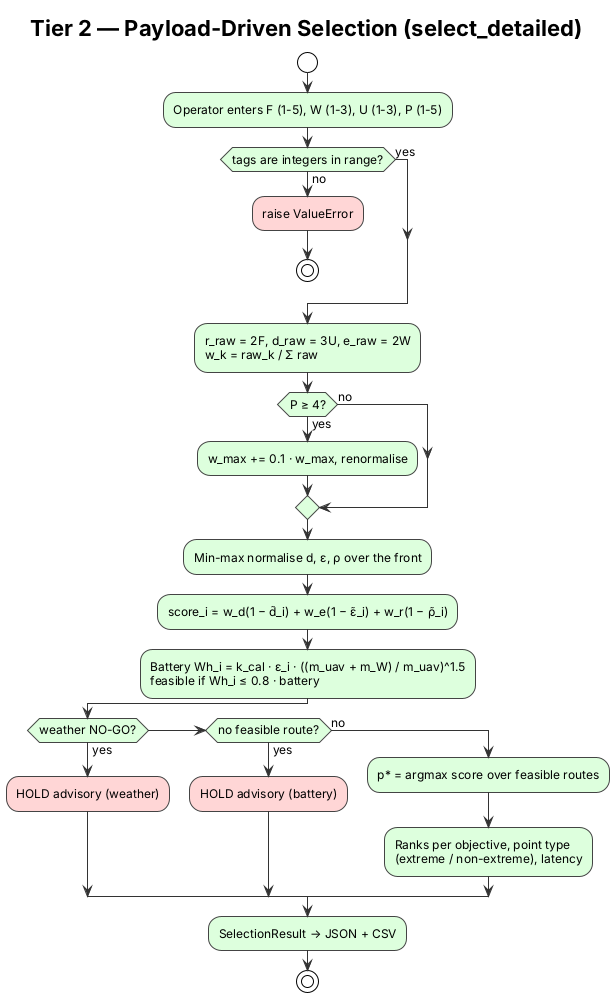
\includegraphics[width=0.56\textwidth]{tier2.png}
\caption{Tier~2 activity flow with validation, feasibility and weather hold}\label{fig:tier2}
\end{figure}

% ------------------------------------------------------------
\subsection{Module 5: Evaluation and Benchmarking}\label{sec:m5}

\subsubsection{Purpose}

Module~5 measures how good a front is and how sensible the Tier~2 picks are. Every
measure is computed per scenario, and the results are written to CSV and JSON so that
each pass of the evaluation cycle can be compared with the last.

\subsubsection{Reference front and normalisation}

There is no known true front for our graphs, so the reference front $\mathcal{R}$ for a
scenario is the non-dominated union of every route found by every method and every
repetition. All metrics are computed in a space normalised by the ideal and nadir points of
$\mathcal{R}$.

\subsubsection{Front quality metrics}

Hypervolume (HV) \cite{r18} is the volume dominated by a front and bounded by a
reference point, here the normalised nadir padded by 10\% ($[1.1, 1.1, 1.1]$). It is
computed exactly in three dimensions by recursive slicing. Larger is better. Inverted
generational distance measures how well a front $A$ covers the reference front:
\begin{equation}
  \mathrm{IGD}(A, \mathcal{R}) = \frac{1}{\lvert\mathcal{R}\rvert}\sum_{r \in \mathcal{R}} \min_{a \in A} \lVert r - a \rVert_2
\end{equation}
Smaller is better, and zero means $A$ contains every reference point. The spread $\Delta$
captures how evenly the points are distributed and how far they reach toward the extremes
of $\mathcal{R}$. Runtime and front size are recorded for every method.

\subsubsection{Tier 2 evidence}

We do not report a Tier~2 ``accuracy'', because there is no ground-truth label for the
correct route. Instead, for each preset the module records the selected route's rank on
each objective, whether it is an extreme or a non-extreme point, the latency, and a
rank-based payload-alignment score
\begin{equation}
  A = \sum_{k \in \{d, \varepsilon, \rho\}} w_k\left(1 - \frac{\mathrm{rank}_k - 1}{K - 1}\right)
\end{equation}
where $K$ is the front size. Because $A$ uses ranks, it does not depend on the min-max
utility that Tier~2 itself maximises. The same score is computed for four competing
selection rules on the same front: the shortest route, the knee point (the point farthest
from the line joining the distance and risk extremes), the largest NSGA-II crowding
distance \cite{r8,r3}, and a fixed equal-weight utility in the style of \cite{r1}.

\subsubsection{Tag sweep and monotonicity}

A sweep runs Tier~2 for all $5 \times 3 \times 3 \times 5 = 225$ tag combinations. It
counts distinct selected routes and non-extreme picks, and it checks monotonicity: raising
$F$ with the other tags fixed must never raise the selected route's risk, raising $U$
must never raise its distance, and raising $W$ must never raise its energy. The target is
zero violations.

\subsubsection{Ablation and component shares}

An ablation runner rebuilds the real-region front with all layers, without wind, without
terrain and without buildings, and draws the edge-risk map and front for each. A
component-share table reports the mean share of each risk component across the front
routes and across the selected routes, which shows which layers actually drive the
choice.

% ------------------------------------------------------------
\subsection{Module 6: Mission Export and Ground-Station Dashboard}\label{sec:m6}

\subsubsection{Mission file generation}

Module~6 turns a selection record into a mission that ArduPilot ground stations can load.
Consecutive lattice waypoints that keep the same bearing and altitude slope (within a
small tolerance) are merged, so a straight run of lattice hops becomes one leg. The file
follows the QGC WPL~110 text format. The first item is home, in the global frame. Every
route waypoint uses frame~3 (\texttt{GLOBAL\_RELATIVE\_ALT}), whose altitude is measured
from home, so the exporter writes
\begin{equation}
  \mathit{alt}_\mathrm{rel} = \mathit{alt}_\mathrm{AMSL} - H_\mathrm{home}
\end{equation}
with $H_\mathrm{home}$ the ground elevation under the first waypoint. The height above
local ground is never written into frame~3, because that would be wrong wherever the
terrain varies. An optional return-to-launch item can
close the mission.

\subsubsection{Operator dashboard}

A small Tkinter dashboard lets an operator load a stored graph and front, type the four
tags, see the selected route drawn on the map, and export the mission file. It covers the
ground-station objective in a minimal form. Two defects are open: the dashboard does not
yet pass the weather reasons to Tier~2, and it can load a graph and a front from different
runs. Both are on the list for the next pass.

% ------------------------------------------------------------
\subsection{Module 7: Simulation and SITL Validation}\label{sec:m7}

\subsubsection{Purpose}

A route that scores well on the graph may still be hard to fly, so Module~7 checks the
flight itself. It flies the Tier~2 route through a three-dimensional model of the delivery area
in Gazebo Harmonic \cite{r24}, with ArduCopter running in software-in-the-loop
\cite{r23}, and compares the flown track with the plan. Figure~\ref{fig:sim} shows the
pipeline. The simulation code imports the planner modules directly; nothing is copied.

\begin{figure}[H]
\centering
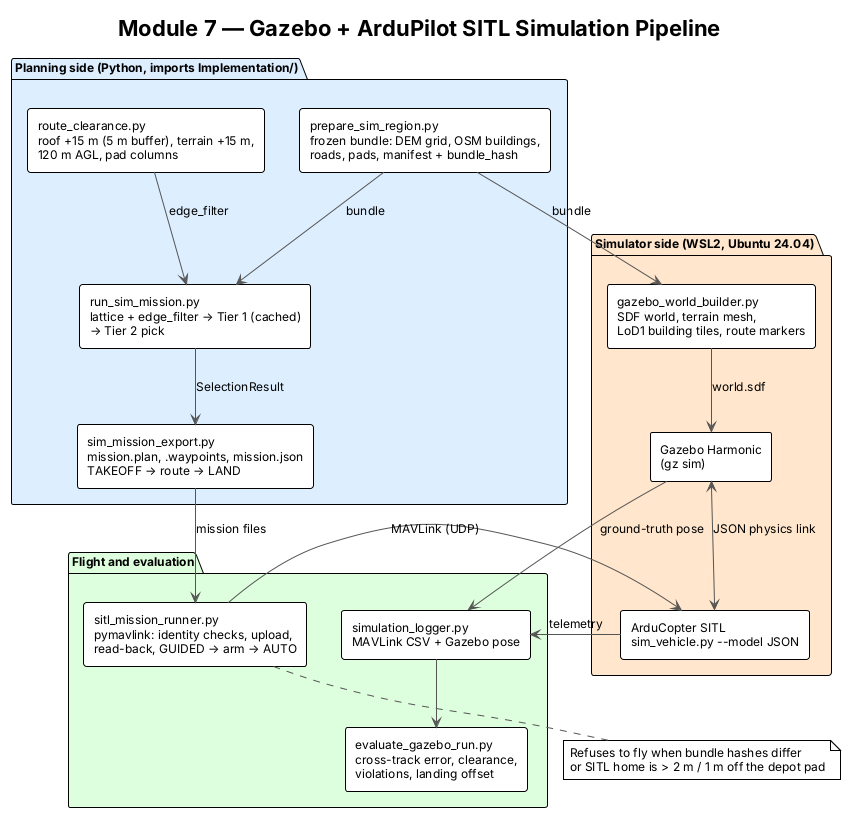
\includegraphics[width=0.85\textwidth]{simulation.png}
\caption{Gazebo and ArduPilot SITL simulation pipeline}\label{fig:sim}
\end{figure}

\subsubsection{Frozen region bundle}

A region is first frozen into a bundle: a terrain grid, OSM buildings with their heights
and the source of each height, roads, the depot and destination pads, and a manifest. The
default simulation region is a 1.5\,km box with a 100\,m lattice. A hash of the bundle is
written into the graph, the front identity, the mission file and the world manifest, and
the runner refuses to fly if they do not match. This stops a mission planned on one
version of the map from being flown in another.

\subsubsection{Hard clearance filter}

Before NAMOA* runs, a clearance checker is passed to the lattice builder as its
\texttt{edge\_filter}. It removes every edge whose buffered segment (5\,m) passes less than
15\,m above a roof, whose terrain clearance sampled every 10\,m drops below 15\,m, or
which exceeds 120\,m above ground. The take-off and landing columns over the pads, and the
connector legs from the pads to the lattice, are checked the same way. Waypoints are
never raised after selection. If a check fails, the planner reports that no feasible
mission exists and writes nothing.

\subsubsection{World building and frame contract}

The world builder writes a Gazebo SDF world with a terrain mesh, LoD1 building tiles
(footprints extruded to their heights), roads, pads and route markers. The world origin
is the depot pad on the ground, with east, north and up axes. SITL is started with its
home at the same point, using the same terrain grid as the planner, so the mission
altitude $\mathit{alt}_\mathrm{AMSL} - H_\mathrm{home}$ means the same height in the
planner, the world and the autopilot. The runner checks this before arming and refuses to
fly if home is more than 2\,m horizontally or 1\,m vertically from the depot pad.

\subsubsection{Mission flight and logging}

The simulation mission is take-off, the route, and a landing on the destination pad, with
no unvalidated return leg. The runner, built on pymavlink, performs identity checks,
uploads the mission, reads it back and compares it with what was sent, switches to
GUIDED, arms, switches to AUTO, and logs telemetry until the vehicle lands and disarms. A
logger records the MAVLink stream and the Gazebo ground-truth pose side by side.

\subsubsection{Flight evaluation}

The evaluator computes the cross-track error of the flown track against the planned
polyline, the minimum clearance above roofs and terrain, any violation of the clearance or
ceiling rules, and the landing offset from the destination pad. It draws the map and
altitude plots and appends a row to a summary table, so runs for different presets and
wind cases can be compared.


% ============================================================
\flowchapter{Implementation}\label{cha:implementation}

The planner is written in Python as flat scripts under \texttt{Implementation/}, one file
per module, plus a configuration file, an environment-data file and entry-point scripts.
The simulation lives under \texttt{Simulation/} and imports the planner modules through
the Python path. This chapter describes how each module is implemented, the data
structures it uses and how it is tested.

\section{Development Environment and Tools}

\begin{table}[H]
\centering\caption{Languages, libraries and tools}\label{tab:tools}\small
\begin{tabularx}{\textwidth}{L{3.6cm} Y}
\toprule
\textbf{Tool} & \textbf{Use in the project}\\
\midrule
Python 3 & All planner, evaluation and simulation-side code\\
NetworkX \cite{r5} & Directed airspace graph, A* baselines, strongly connected components\\
NumPy & Vectorised node environment, dominance checks, metrics\\
Shapely 2 (STRtree) & Spatial indexes for buildings, zones, water and population classes\\
GeoPandas, pyogrio, OSMnx \cite{r4} & OSM layer parsing and GeoPackage caching\\
requests & Open-Meteo, OpenTopography and Overpass HTTP calls\\
Matplotlib & Graph, front, route and benchmark figures\\
Tkinter & Operator dashboard\\
pymavlink, MAVLink \cite{r7} & Mission upload, read-back and flight control in SITL\\
Gazebo Harmonic, ArduPilot SITL & Three-dimensional city simulation and autopilot\\
unittest & Planner and simulation test suites (offline, keyless)\\
PlantUML, \LaTeX & Diagrams and this report\\
\bottomrule
\end{tabularx}
\end{table}

All tunable constants (region, flight heights, wind coefficients, risk weights, battery
and mass values, drift thresholds, Overpass endpoints) live in one file,
\texttt{config.py}, so an experiment changes a value in one place. API keys are read from
a \texttt{.env} file by the entry-point scripts only, so the test suites never need a key
or a network connection.

\section{Code Organisation}

\begin{table}[H]
\centering\caption{Source files and the modules they implement}\label{tab:files}\small
\begin{tabularx}{\textwidth}{L{4.85cm} L{1.5cm} Y}
\toprule
\textbf{File} & \textbf{Module} & \textbf{Role}\\
\midrule
\texttt{config.py} & all & Every tunable constant\\
\texttt{env\_data.py} & 1 & Weather, DEM providers, OSM layers, spatial indexes, \texttt{.env} loader\\
\texttt{overpass\_client.py} & 1 & Multi-endpoint Overpass fetch with retry\\
\texttt{module1\_graph\_builder.py} & 1 & Synthetic and lattice builders, cost pipeline\\
\texttt{module2\_tier1\_moastar.py} & 2 & NAMOA* engine, dominance helpers, thinning\\
\texttt{pareto\_store.py} & 2 & Front store, graph hash, drift, region runs\\
\texttt{module3\_baselines.py} & 3 & A* variants, weighted-sum A*, MOPSO\\
\texttt{module4\_tier2\_payload.py} & 4 & Weight bridge, selector, feasibility, export\\
\texttt{module5\_evaluation.py} & 5 & HV, IGD, spread, Tier~2 evidence, sweep\\
\texttt{run\_benchmarks.py}, \texttt{run\_ablation.py} & 5 & Benchmark and ablation runners\\
\texttt{mission\_export.py}, \texttt{dashboard.py} & 6 & QGC WPL~110 export, operator UI\\
\texttt{run\_demo\_syn.py}, \texttt{run\_demo\_osm.py} & 1--4 & End-to-end demos with figures\\
\texttt{Simulation/*.py} & 7 & Bundle, clearance, world, mission, runner, logger, evaluator\\
\bottomrule
\end{tabularx}
\end{table}

Figure~\ref{fig:classes} shows the main classes and how they relate.

\begin{figure}[H]
\centering
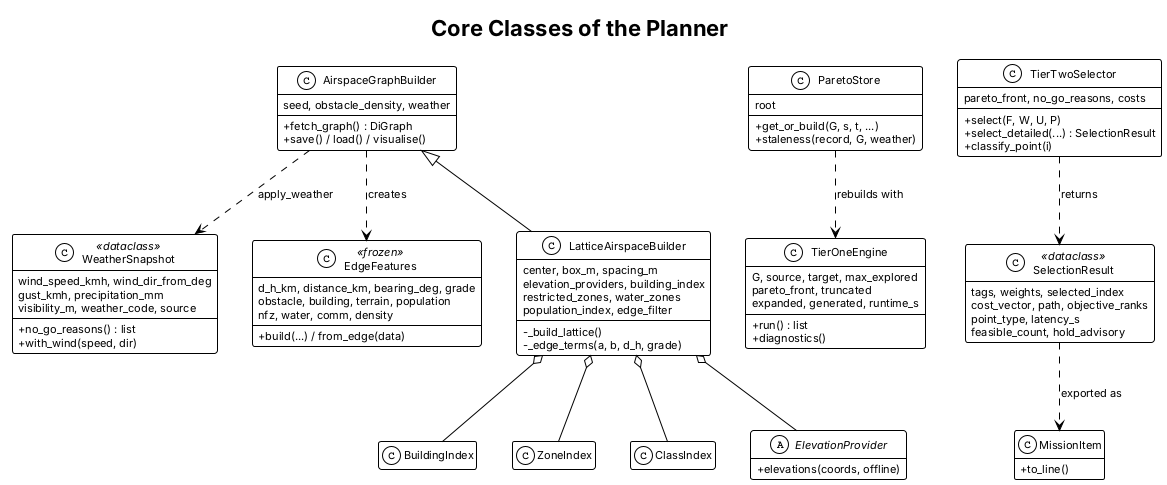
\includegraphics[width=\textwidth]{classes.png}
\caption{Core classes of the planner}\label{fig:classes}
\end{figure}

\section{Module 1: Airspace Graph Builder}

\subsection{Weather and terrain data}

\texttt{WeatherSnapshot} is a dataclass holding wind speed, direction, gust, rain,
visibility, the WMO code, the observation time and the source of the data (live,
power-law, cache, override, synthetic or calm). Its constructor normalises the direction
to $[0, 360)$ and forces the gust to be at least the mean wind. \texttt{no\_go\_reasons()}
implements the weather gate, and \texttt{with\_wind()} produces the override used for
controlled wind experiments. \texttt{fetch\_weather()} never raises: it tries the live API,
then the cache, then calm air.

Elevation providers share one interface, the \texttt{elevations()} method of
\texttt{ElevationProvider}, which looks up the disk cache first and only sends uncached points to the service.
\texttt{fetch\_elevations()} walks the provider list and reports which provider supplied
the values, so the console always says where the terrain came from.

\subsection{OSM layers and spatial indexes}

\texttt{fetch\_osm\_layers()} queries the Overpass endpoints in turn (with two attempts each,
a pause on HTTP 406, 429 and 5xx, and a cap on \texttt{Retry-After} waits) and caches the
result as GeoPackage. A failed fetch returns empty layers and the run still completes, so
the console prints the layer counts and they must be checked before a result is called
real. \texttt{build\_layer\_indexes()} projects every geometry into the local metric frame
and builds the indexes. \texttt{BuildingIndex} answers four vectorised queries over arrays
of points: the tallest building in a square cell, the building density and mean height of
a cell, the tallest building directly under a point, and the tallest building within a
radius. \texttt{ZoneIndex} answers containment, clipped distance and segment-intersection
queries, and \texttt{ClassIndex} returns the highest population class covering a point.

\subsection{Lattice builder}

\texttt{LatticeAirspaceBuilder.\_build\_lattice()} works on whole arrays. It builds the
node coordinates with a NumPy mesh grid, converts them to latitude and longitude in one
call, fetches all ground elevations in one batched provider call and computes the
building statistics for all cells at once. The blocked mask
$(\mathrm{AGL} > 120) \lor \mathrm{inNFZ}$ is a single array expression. Candidate edges
are collected first, and the NFZ test on all of them runs as one vectorised
segment-intersection query. The \texttt{edge\_filter} hook is then applied, the static
terms are computed per edge by \texttt{\_edge\_terms()}, and the graph is reduced to its
largest strongly connected component. Build statistics (provider, layer counts, blocked
nodes, removed edges) are stored on the graph for the report and the console.

Each edge's static features are held in a frozen dataclass, \texttt{EdgeFeatures}, which
clips every risk term to $[0,1]$ when it is created. Weather-dependent values are never
stored in it. The cost pipeline is a pair of pure functions:

\begin{lstlisting}[language=Python, caption={Wind decomposition and energy (module1\_graph\_builder.py)}, label={lst:wind}]
def wind_components(bearing_deg, speed_kmh, dir_from_deg):
    rel = math.radians(bearing_deg - dir_from_deg)
    return speed_kmh * math.cos(rel), speed_kmh * abs(math.sin(rel))

def energy_cost(f: EdgeFeatures, w: WeatherSnapshot) -> float:
    hw, cw = wind_components(f.bearing_deg, w.wind_speed_kmh,
                             w.wind_dir_from_deg)
    factor = (1.0 + abs(f.grade)
              + cfg.BETA_HEAD * max(0.0, hw) / cfg.V_CRUISE_KMH
              + cfg.BETA_CROSS * cw / cfg.V_CRUISE_KMH)
    return f.distance_km * factor
\end{lstlisting}

The function \texttt{apply\_weather()} loops over the edges, rebuilds the
static features of each edge from its stored attributes, and writes \texttt{energy}, \texttt{rho},
\texttt{risk}, \texttt{risk\_components}, \texttt{cost} and \texttt{time\_s}. It then
writes the snapshot and the gate result to \texttt{G.graph}.

\subsection{Main parameters}

\begin{table}[H]
\centering\caption{Main Module~1 parameters (\texttt{config.py})}\label{tab:params}\small
\begin{tabularx}{\textwidth}{L{4.4cm} L{2.4cm} Y}
\toprule
\textbf{Parameter} & \textbf{Value} & \textbf{Meaning}\\
\midrule
\texttt{CENTER\_LAT, CENTER\_LON} & 12.9830, 80.2594 & Centre of the example region\\
\texttt{BOX\_M}, \texttt{LATTICE\_SPACING\_M} & 6000\,m, 200\,m & Lattice extent and spacing\\
\texttt{H\_CRUISE\_AGL}, \texttt{CLEARANCE} & 60\,m, 15\,m & Cruise height, margin above roofs\\
\texttt{H\_MAX\_AGL} & 120\,m & Legal ceiling\\
\texttt{V\_CRUISE\_KMH} & 36\,km/h & Airspeed used in the wind terms\\
\texttt{BETA\_HEAD}, \texttt{BETA\_CROSS} & 0.40, 0.15 & Headwind and crosswind energy coefficients\\
\texttt{V\_MAX\_SAFE\_KMH}, \texttt{K\_GUST} & 40\,km/h, 0.5 & Wind risk saturation, gust weight\\
\texttt{ALPHA\_SHEAR} & 0.25 & Power-law shear exponent\\
\texttt{EDGE\_SAMPLE\_STEP\_M} & 25\,m & Along-edge sampling step\\
\texttt{NFZ\_SOFT\_LAMBDA\_M} & 150\,m & Decay length of the no-fly buffer\\
\texttt{NO\_GO\_GUST\_KMH} & 45\,km/h & Gust limit (provisional)\\
\bottomrule
\end{tabularx}
\end{table}

\subsection{Entry points}

\texttt{run\_demo\_osm.py} runs the lattice pipeline end to end. Its options cover the
experiments in this report: \texttt{--offline} (cache or fixtures only),
\texttt{--wind-override SPEED DIR} (controlled wind), \texttt{--no-terrain},
\texttt{--no-buildings} and \texttt{--no-risk-layers} (ablation), \texttt{--refresh}
(force a new front), \texttt{--front-max N} (thinning), \texttt{--box-km} and
\texttt{--spacing-m} (graph size), and \texttt{--payload F W U P} or \texttt{--preset}
(Tier~2 input). \texttt{run\_demo\_syn.py} does the same on the synthetic graph.

\section{Module 2: Tier 1 Engine and Front Store}

\subsection{Label table}

\texttt{TierOneEngine.run()} keeps the label table as four parallel Python lists
(\texttt{lab\_node}, \texttt{lab\_g}, \texttt{lab\_parent}, \texttt{lab\_dead}) indexed by
label id, and a dictionary from node to the ids of its live labels. The open list is a
binary heap of (priority, sequence number, label id); the sequence number breaks ties so
that runs are deterministic. Heuristic vectors are cached per node. The front is kept
twice: as a list of label ids and as a NumPy array, so that the check ``does the front
weakly dominate this vector'' is one vectorised comparison instead of a Python loop. When
the search ends, each front label is turned into a path by following parent ids, and the
routes are sorted by cost vector.

\subsection{Diagnostics}

After a run the engine exposes \texttt{truncated}, \texttt{expanded}, \texttt{generated},
\texttt{runtime\_s} and the front size through \texttt{diagnostics()}. The default cap is
200,000 expansions; the benchmark runner raises it per scenario (80,000, 180,000 and
260,000 for S1, S2 and S3).

\subsection{Front store}

\texttt{ParetoStore} writes one indented JSON file per (region, source, target) under
\texttt{pareto\_front\_storage/fronts/}. \texttt{graph\_hash()} sorts the edges, formats the
twelve static attributes of each to five decimals and feeds them to SHA-256.
\texttt{weather\_drift()} compares the stored snapshot with the new one and returns a list
of human-readable reasons, which \texttt{get\_or\_build()} prints before rebuilding. The
function returns the record, a flag saying whether it was rebuilt, and the reasons, so a
caller can tell a reused front from a fresh one.

\section{Module 3: Baselines}

Each baseline returns a \texttt{BaselineResult} with the method name, its routes as
(cost vector, path) pairs, the runtime and its settings. The A* variants call
\texttt{networkx.astar\_path} with a weight function that reads the chosen objective from
the edge. \texttt{route\_cost()} re-sums a path's cost on the graph, and
\texttt{is\_valid\_route()} checks that the path starts and ends at the right nodes, that
every edge exists and that no node repeats; every MOPSO particle is checked with it. The
MOPSO archive is updated through the same \texttt{update\_pareto\_front()} helper that
Tier~1 uses, so both methods apply exactly the same dominance rule.

\section{Module 4: Tier 2 Selector}

The weight bridge is a direct transcription of Equations~(\ref{eq:raw})
and~(\ref{eq:weights}):

\begin{lstlisting}[language=Python, caption={Weight derivation (module4\_tier2\_payload.py)}, label={lst:weights}]
def derive_weights(F: int, W: int, U: int) -> tuple:
    F = _validate_integer_tag("F", F, 1, 5)
    W = _validate_integer_tag("W", W, 1, 3)
    U = _validate_integer_tag("U", U, 1, 3)
    r_raw, d_raw, e_raw = F * 2, U * 3, W * 2
    total = r_raw + d_raw + e_raw
    return r_raw / total, d_raw / total, e_raw / total
\end{lstlisting}

\texttt{TierTwoSelector} computes the per-objective minima and maxima of the front once,
in its constructor, so each selection only normalises and scores. A degenerate objective
(all routes equal) normalises to zero instead of dividing by zero.
\texttt{select\_detailed()} validates the tags, derives and amplifies the weights, scores
every route, filters by battery feasibility with \texttt{route\_energy\_wh()}, applies the
weather gate, and builds a \texttt{SelectionResult}. The waypoints in the result carry
node id, latitude, longitude, altitude above sea level and height above ground, taken
from the graph. The record is written to \texttt{outputs/tier2/selection\_<name>.json} and
\texttt{.csv}. The simpler \texttt{select()} is kept for the demos and the sweep; it raises
\texttt{WeatherNoGo} under a no-go but does not apply the battery filter, which is a known
gap to be closed by routing all callers through \texttt{select\_detailed()}.

\section{Module 5: Evaluation}

\texttt{module5\_evaluation.py} contains the metric functions and the Tier~2 evidence
functions. The exact hypervolume slices the normalised points along the first objective
and recurses on the remaining two. \texttt{build\_reference\_front()} takes the routes of
every method and keeps the non-dominated union. \texttt{tier2\_evidence()} runs the four
presets and the four competing pickers on one front, and \texttt{tier2\_sweep()} runs all
225 combinations.

\texttt{run\_benchmarks.py} builds the S1, S2 and S3 graphs from fixed seeds (101, 202,
303), runs NAMOA*, the A* baselines and MOPSO, and writes \texttt{benchmark\_metrics.csv},
\texttt{tier2\_evidence.csv} and bar charts of HV, IGD, spread, front size and runtime to
\texttt{outputs/benchmarks/}. It takes \texttt{--scenario}, \texttt{--mopso-repetitions}
(default 30), \texttt{--swarm-size} (100), \texttt{--iterations} (200),
\texttt{--archive-size} and \texttt{--smoke}. \texttt{run\_ablation.py} produces the
ablation fronts, edge-risk maps and component maps in \texttt{outputs/ablation/}.

\section{Module 6: Mission Export and Dashboard}

\texttt{mission\_export.py} represents each mission line as a \texttt{MissionItem}
(index, current flag, frame, command, four parameters, latitude, longitude, altitude,
auto-continue) and serialises it as a tab-separated QGC WPL~110 line. Collinear points are
merged when the bearing changes by at most 2$^\circ$ and the altitude slope by at most
0.5. A parser reads the file back, which the tests use to check that export and import
agree. \texttt{dashboard.py} is a single Tkinter window with fields for the four tags, an
embedded Matplotlib map and an export button.

\section{Module 7: Simulation}

The simulation side is run in WSL2 (Ubuntu 24.04) with Gazebo Harmonic, the ArduPilot
Gazebo plugin and an ArduCopter SITL build. A delivery is simulated in five steps:

\begin{enumerate}[label=\arabic*.]
  \item \texttt{prepare\_sim\_region.py --strict} freezes the region bundle from live OSM
  and DEM data; \texttt{--strict} refuses the hand-made test fixtures.
  \item \texttt{gazebo\_world\_builder.py <region>} writes the world, meshes and the
  matching SITL command line.
  \item \texttt{run\_sim\_mission.py} with \texttt{--preset}, \texttt{--payload},
  \texttt{--all-presets} or \texttt{--baseline} plans the mission and writes
  \texttt{mission.plan}, \texttt{.waypoints} and \texttt{mission.json}. A tag-only change
  reuses the stored front and does not rerun NAMOA*.
  \item The world is launched with the route markers, SITL is started with
  \texttt{--custom-location} at the depot, and \texttt{sitl\_mission\_runner.py} flies the
  mission.
  \item \texttt{evaluate\_gazebo\_run.py} computes the flight metrics and plots.
\end{enumerate}

The runner handles two ArduPilot version details. ArduCopter 4.7 and later name the
waypoint speed parameter \texttt{WP\_SPD} (m/s) instead of \texttt{WPNAV\_SPEED} (cm/s), so the
runner sets whichever one exists, and ArduPilot echoes \texttt{DO\_CHANGE\_SPEED}
with frame~0 on read-back, which the comparison accepts.

\section{Testing}

Both code bases have offline unit-test suites that need no network and no API key. The
planner suite has about 220 tests and the simulation suite 45.
Table~\ref{tab:tests} lists what they cover.

\small
\begin{xltabular}{\textwidth}{L{5.6cm} Y}
\caption{Test suites and what they verify}\label{tab:tests}\\
\toprule
\textbf{Test file} & \textbf{What it checks}\\
\midrule
\endfirsthead
\multicolumn{2}{l}{\small\itshape Table \thetable\ (continued)}\\
\toprule
\textbf{Test file} & \textbf{What it checks}\\
\midrule
\endhead
\bottomrule
\endlastfoot
\texttt{test\_wind.py} & Headwind sign (wind from 90$^\circ$ is a headwind for an east-bound edge), crosswind, power-law shear, hourly row selection\\
\texttt{test\_lattice.py} & Lattice size, 8-neighbour edges, east-bound edges cost more than west-bound under an east wind\\
\texttt{test\_terrain.py} & DEM provider chain and cache, node altitude rule, every node within 120\,m AGL\\
\texttt{test\_risk.py} & Risk components in $[0,1]$, NFZ node and edge removal, soft buffer, weather gate\\
\texttt{test\_tier1\_front.py} & NAMOA* front equals a brute-force front over all simple paths on a small graph; no route dominates another; every path valid\\
\texttt{test\_store.py} & Reuse, expiry, graph-hash change, each drift threshold, identity check\\
\texttt{test\_tier2\_payload.py}, \texttt{test\_tier2\_hardening.py} & Weight formula, amplification, non-extreme pick for mixed cargo on a stored lattice front, monotonicity, validation errors, latency under 1\,s, battery HOLD\\
\texttt{test\_evaluation\_metrics.py} & HV, IGD, spread on hand-computed cases; alignment score; pickers\\
\texttt{test\_mission\_export.py} & QGC WPL~110 round trip, collinear merge, frame~3 altitude relative to home\\
\texttt{test\_ablation.py}, \texttt{test\_overpass.py}, \texttt{test\_dotenv.py}, \texttt{test\_dashboard\_helpers.py} & Ablation smoke run, Overpass retry and parsing, key loading, dashboard helpers\\
\texttt{Simulation/tests/*} & Bundle loading and frames, clearance checker, mission export (TAKEOFF $\rightarrow$ route $\rightarrow$ LAND), world builder geometry\\
\end{xltabular}
\normalsize


% ============================================================
\flowchapter{Results and Discussion}\label{cha:results}

This chapter reports the results the system currently produces. The numbers come from the
first pass of the evaluation cycle described in Chapter~\ref{cha:queries}, from a
controlled wind experiment run for this report, from the ablation runner, and from the
first SITL flights. They are preliminary in a specific sense: MOPSO was run at reduced
settings, the risk weights and battery constants are not yet calibrated, and the
synthetic density labels have a known defect. We state the caveats next to each result
so that the reader can judge how far it can be pushed.

\section{Experimental Setup}

\begin{table}[H]
\centering\caption{Scenarios used in this chapter}\label{tab:scenarios}\small
\begin{tabularx}{\textwidth}{L{3.2cm} L{2.2cm} Y}
\toprule
\textbf{Scenario} & \textbf{Size} & \textbf{Description}\\
\midrule
S1 small sparse & 50 nodes & Synthetic grid, seed 101, weather seeded\\
S2 medium & 196--200 nodes & Synthetic grid, seed 202, weather seeded (benchmark) or set explicitly (wind experiment)\\
S3 large dense & 500 nodes & Synthetic grid, seed 303, weather seeded\\
Lattice & 893 nodes, 6,752 edges & 6\,km box, 200\,m spacing, offline fixture layers (ablation)\\
Flat lattice & 225 nodes, 1,624 edges & 3\,km box, 200\,m spacing, no layers (directional cost check)\\
\bottomrule
\end{tabularx}
\end{table}

All runs used the current code on a laptop-class CPU. In the first
benchmark pass MOPSO used 24 particles, 30 iterations and 2 repetitions per scenario; the
report-scale run (100, 200, 30) is the next step of the cycle.

\section{Tier 1 Front Quality Against the Baselines}

Table~\ref{tab:bench} gives the first-pass benchmark. Hypervolume (HV) and IGD are
computed in normalised objective space against the union reference front of each scenario.

\begin{table}[H]
\centering\caption{First-pass benchmark on synthetic scenarios (HV higher is better; IGD
and $\Delta$ lower are better)}\label{tab:bench}\small
\begin{tabular}{l l r r r r r}
\toprule
\textbf{Scenario} & \textbf{Method} & \textbf{Front} & \textbf{Time (s)} & \textbf{HV} & \textbf{IGD} & $\boldsymbol{\Delta}$\\
\midrule
\multirow{5}{*}{S1 (50)}  & NAMOA* (Tier 1) & 2   & 0.003  & 0.131  & 0.000 & 0.000\\
                          & A* distance     & 1   & $<$0.001 & 0.121 & 0.866 & --\\
                          & A* energy       & 1   & $<$0.001 & 0.121 & 0.866 & --\\
                          & A* risk         & 1   & $<$0.001 & 0.011 & 0.866 & --\\
                          & MOPSO           & 2   & 0.363  & 0.131  & 0.000 & 0.000\\
\midrule
\multirow{5}{*}{S2 (200)} & NAMOA* (Tier 1) & 16  & 0.162  & 1.2065 & 0.000 & 1.001\\
                          & A* distance     & 1   & $<$0.001 & 0.107 & 1.021 & --\\
                          & A* energy       & 1   & $<$0.001 & 1.083 & 0.648 & --\\
                          & A* risk         & 1   & $<$0.001 & 0.011 & 0.887 & --\\
                          & MOPSO           & 12  & 1.505  & 1.2061 & 0.017 & 1.027\\
\midrule
\multirow{5}{*}{S3 (500)} & NAMOA* (Tier 1) & 115 & 33.761 & 1.1235 & 0.000 & 0.666\\
                          & A* distance     & 1   & 0.001  & 0.062  & 0.861 & --\\
                          & A* energy       & 1   & 0.002  & 0.674  & 0.442 & --\\
                          & A* risk         & 1   & 0.002  & 0.013  & 1.116 & --\\
                          & MOPSO           & 38  & 4.326  & 1.1146 & 0.043 & 0.814\\
\bottomrule
\end{tabular}
\end{table}

NAMOA* has an IGD of zero in every scenario, which means its front contains every point of
the reference front. That is what an exact method should give, and it confirms that the
pruning rules do not throw away non-dominated routes. MOPSO recovers 12 of the 16 routes
on S2 and 38 of the 115 on S3, and its HV is close to that of NAMOA* (a gap of 0.0004 on S2
and 0.009 on S3). The gap is small because MOPSO's archive still spans the extremes, even
though it misses many interior points. Interior points are exactly the ones Tier~2 needs
for mixed payloads, so the IGD and front-size columns matter more for this project than
the HV column. NAMOA* also spreads its points more evenly ($\Delta$ of 0.666 against
0.814 on S3).

The single-objective A* routes reach high HV only when their one objective happens to
dominate the volume, as A* energy does on S2. They cannot cover the front, and their IGD
stays between 0.44 and 1.12.

Exactness has a cost. On S3, NAMOA* took 33.8\,s against MOPSO's 4.3\,s. Tier~1 runs once
per region and weather window, not once per mission, so this is acceptable, but it is a
target for the next cycle (front thinning, a tighter heuristic and a coarser lattice in
open areas). Figures~\ref{fig:bench-hv} and~\ref{fig:bench-time} plot the same data.

\begin{figure}[H]
\centering
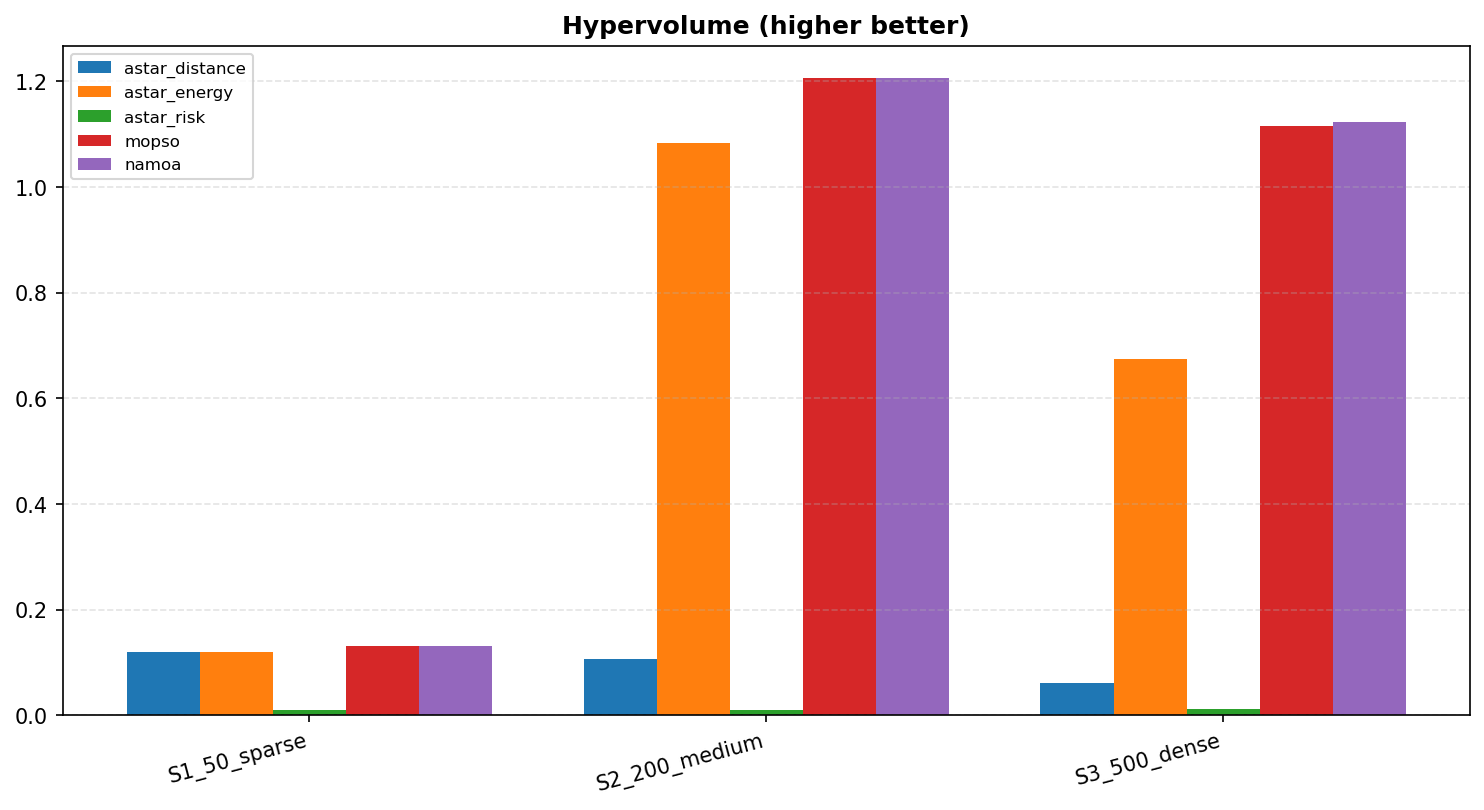
\includegraphics[width=0.78\textwidth]{benchmark_hv.png}
\caption{Hypervolume per method and scenario (first pass)}\label{fig:bench-hv}
\end{figure}

\begin{figure}[H]
\centering
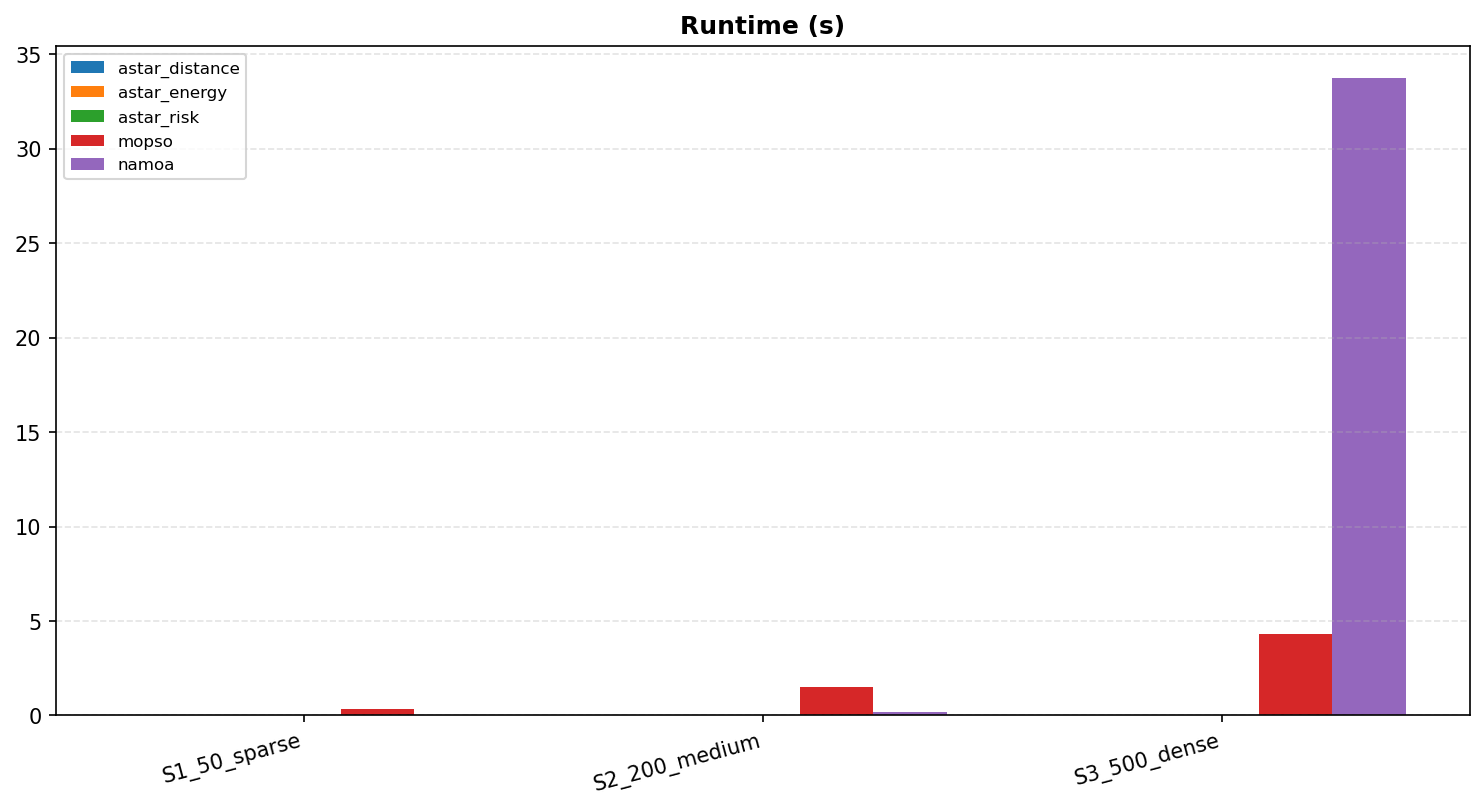
\includegraphics[width=0.78\textwidth]{benchmark_runtime.png}
\caption{Runtime per method and scenario (first pass)}\label{fig:bench-time}
\end{figure}

\section{Effect of Wind Speed and Direction}\label{sec:res-wind}

This experiment isolates the wind model. The S2 synthetic graph (196 nodes, 1,404
edges, seed 202) was costed under calm air and under a 25\,km/h wind with 35\,km/h gusts
blowing from each of eight compass directions. Nothing else changed: the same graph, the
same static layers, the same source and target. Table~\ref{tab:wind} shows the result.

\begin{table}[H]
\centering\caption{Effect of wind direction on the S2 front (25\,km/h wind, 35\,km/h gust)}\label{tab:wind}\footnotesize\setlength{\tabcolsep}{4pt}
\begin{tabular}{l r r r r c r}
\toprule
\textbf{Wind from} & \textbf{Front} & \textbf{Labels} & \textbf{Min $\boldsymbol{\varepsilon}$} & \textbf{Min $\boldsymbol{\rho}$} & \textbf{Fragile pick $(d, \varepsilon, \rho)$} & \textbf{Distinct}\\
\midrule
Calm          & 36 & 869  & 24.41 & 0.07 & (26.78, 26.92, 0.11) & 4\\
0$^\circ$ (N)   & 14 & 1019 & 31.01 & 3.24 & (26.16, 32.82, 3.40) & 2\\
45$^\circ$ (NE) & 6  & 545  & 31.34 & 1.89 & (26.16, 33.63, 1.89) & 2\\
90$^\circ$ (E)  & 11 & 876  & 30.94 & 3.31 & (26.16, 32.75, 3.45) & 2\\
135$^\circ$ (SE)& 14 & 1100 & 27.13 & 4.27 & (26.16, 29.59, 4.42) & 2\\
180$^\circ$ (S) & 14 & 989  & 26.18 & 3.24 & (26.16, 27.99, 3.40) & 2\\
225$^\circ$ (SW)& 6  & 482  & 24.58 & 1.89 & (26.16, 26.87, 1.89) & 2\\
270$^\circ$ (W) & 11 & 801  & 26.22 & 3.31 & (26.16, 28.03, 3.45) & 2\\
315$^\circ$ (NW)& 14 & 1084 & 27.21 & 4.27 & (26.16, 29.67, 4.42) & 2\\
\bottomrule
\end{tabular}
\end{table}

The first observation is that direction alone matters a great deal. At the same speed,
the cheapest route on the front needs 24.58 energy units with the wind from the south-west
and 31.34 with it from the north-east, a difference of 27.5\%. A planner that used wind
speed without direction could not see this.

The risk and energy objectives also respond to different properties of the wind.
Opposite directions (0$^\circ$ and 180$^\circ$, or 45$^\circ$ and 225$^\circ$) give the
same minimum risk, because crosswind depends only on the axis of the wind. They give very
different minimum energy, because the headwind penalty depends on which way along that
axis the drone is flying. This is the behaviour Equation~(\ref{eq:hwcw}) predicts, and it
is why both components are needed.

Finally, wind changes the shape of the front as well as its position. The front shrinks from
36 routes in calm air to between 6 and 14, and the four presets land on only two
distinct routes. Under a steady wind, edges with strong crosswind are both costlier and
riskier, so energy and risk become correlated and there are fewer real trade-offs left.
The fragile medical pick stays the lowest-risk option on every front, but its energy
varies from 26.87 to 33.63 with direction. Whether the collapse to two picks is the right
behaviour or an artefact of min-max normalisation on a short front is one of the questions
the next evaluation pass has to settle. Figure~\ref{fig:wind-sweep} repeats the experiment
in 15$^\circ$ steps.

\begin{figure}[H]
\centering
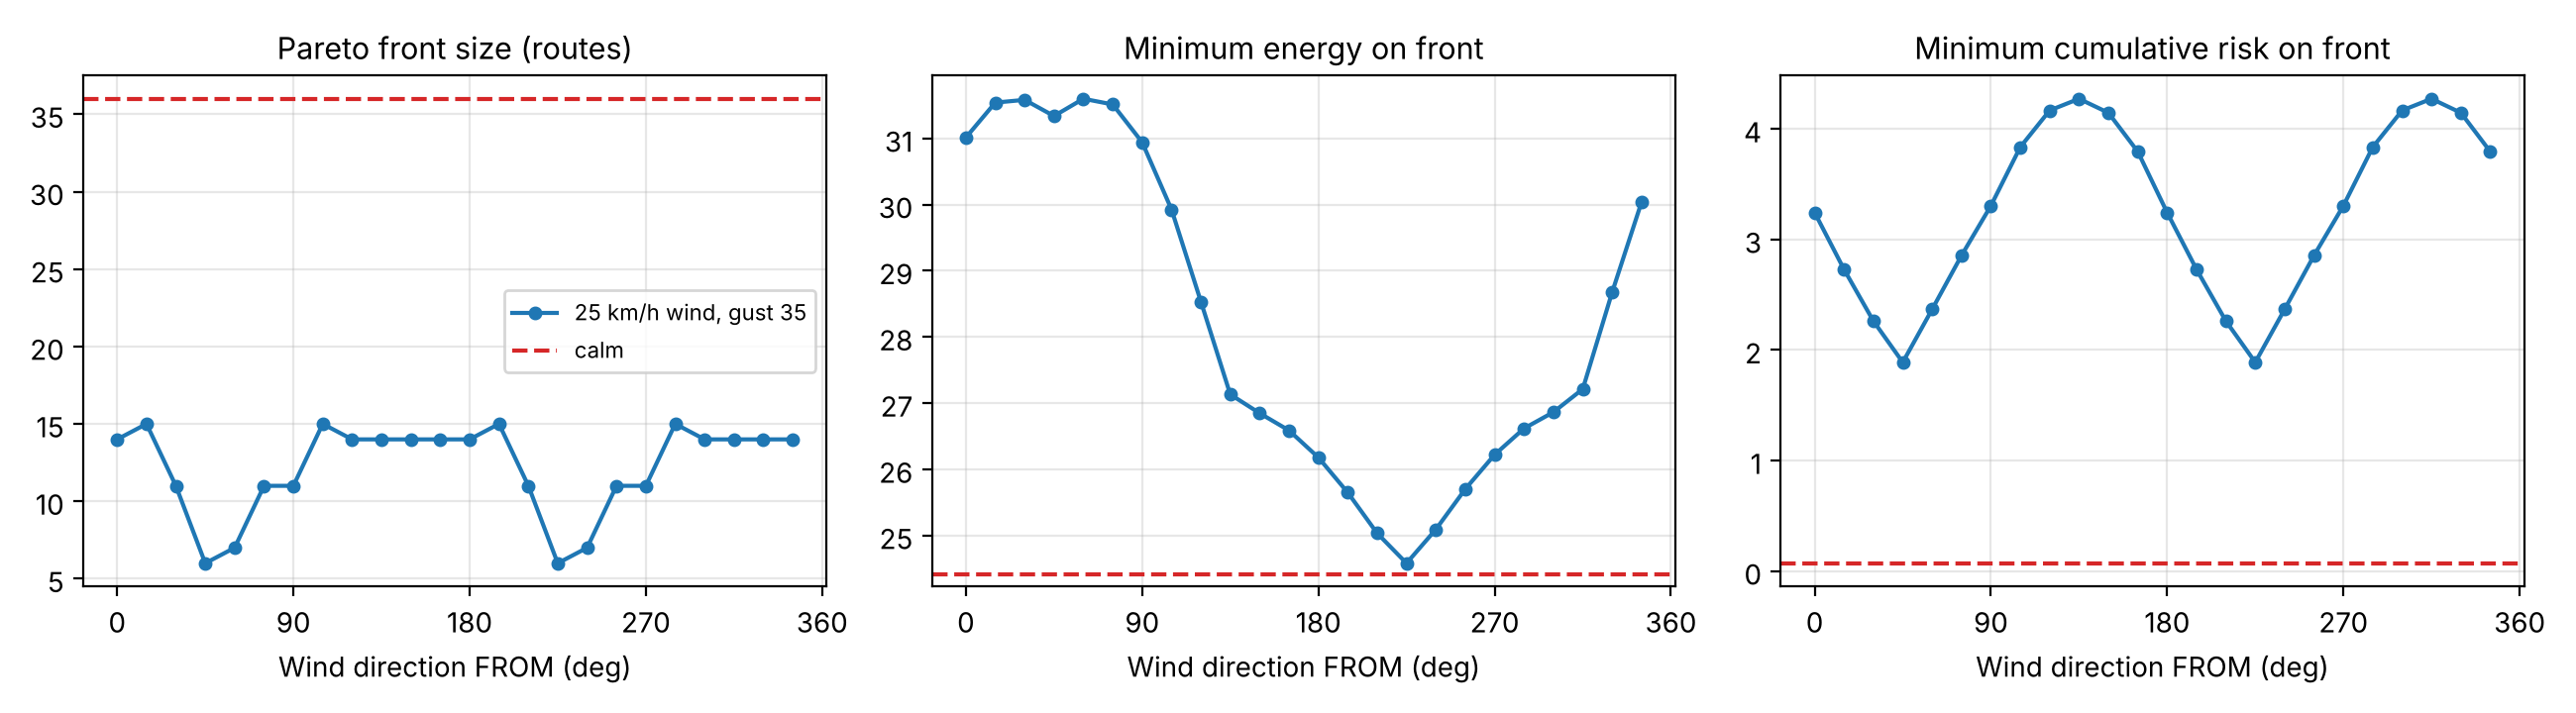
\includegraphics[width=\textwidth]{wind_direction_sweep.png}
\caption{Front size, minimum energy and minimum risk on S2 as a 25\,km/h wind turns
through 360$^\circ$; the dashed line is calm air}\label{fig:wind-sweep}
\end{figure}

The same effect shows up edge by edge. Table~\ref{tab:dir-edges} lists the mean energy per
kilometre and the mean edge risk score by heading on a flat 3\,km lattice with no other
layers, under a 25\,km/h wind from the east.

\begin{table}[H]
\centering\caption{Directional edge costs on a flat lattice, 25\,km/h wind from 90$^\circ$}\label{tab:dir-edges}\small
\begin{tabular}{l r r r r r r r r}
\toprule
\textbf{Edge heading} & 0$^\circ$ & 45$^\circ$ & 90$^\circ$ & 135$^\circ$ & 180$^\circ$ & 225$^\circ$ & 270$^\circ$ & 315$^\circ$\\
\midrule
$\varepsilon / d$       & 1.104 & 1.270 & 1.278 & 1.270 & 1.104 & 1.074 & 1.000 & 1.074\\
$\rho_\mathrm{edge}$    & 0.225 & 0.170 & 0.038 & 0.170 & 0.225 & 0.170 & 0.038 & 0.170\\
\bottomrule
\end{tabular}
\end{table}

East-bound edges fly into the wind and cost 27.8\% more energy per kilometre than
west-bound edges, which fly with it and cost exactly their distance because tailwind earns
no credit. North- and south-bound edges take the full crosswind and carry six times the
risk score of east--west edges, whose remaining 0.038 comes only from the gust term. On a
flat lattice with no obstacles the front still has a single route, since the straight
diagonal is best on every objective. Trade-offs need the wind to interact with terrain,
buildings or restricted zones, which is what the next two results show.

\section{Contribution of Each Risk Layer}

The ablation runner rebuilt the lattice front with all layers and with
wind, terrain or buildings removed, under a 30\,km/h wind from the south-west. These runs
used the offline fixture layers, which are hand-made test data shaped like the real
region, so the numbers show how each layer acts on the planner rather than real-world
values. The live-data run is part of the next cycle.

\begin{table}[H]
\centering\caption{Ablation on the 6\,km lattice (fixture layers, 30\,km/h wind from 225$^\circ$)}\label{tab:ablation}\small
\begin{tabular}{l r r r r r r}
\toprule
\textbf{Variant} & \textbf{Front} & \textbf{Time (s)} & \textbf{Min $\boldsymbol{\varepsilon}$} & \textbf{Min $\boldsymbol{\rho}$} & \textbf{Max $\boldsymbol{\rho}$} & \textbf{Mean $\boldsymbol{\rho_\mathrm{edge}}$}\\
\midrule
All layers   & 196 & 11.35 & 8.82 & 8.85 & 13.12 & 0.199\\
No wind      & 205 & 5.38  & 7.84 & 0.10 & 4.24  & 0.061\\
No terrain   & 56  & 1.36  & 8.81 & 8.81 & 13.08 & 0.198\\
No buildings & 190 & 8.32  & 8.82 & 8.85 & 12.26 & 0.192\\
\bottomrule
\end{tabular}
\end{table}

Wind is the largest single driver of risk in this setting. Removing it lowers the mean
edge risk from 0.199 to 0.061 and the risk of the safest route from 8.85 to 0.10, and it
lowers the minimum energy by 11\%. Terrain mostly drives the size of the front: without
grades there are far fewer distinct trade-offs (56 routes against 196), because altitude
changes are what separate otherwise similar paths. Buildings raise the upper end of the
risk range. Figure~\ref{fig:risk-maps} shows the edge-risk maps for the four variants;
the hole near the top centre is a restricted zone whose nodes and crossing edges were
removed.

\begin{figure}[H]
\centering
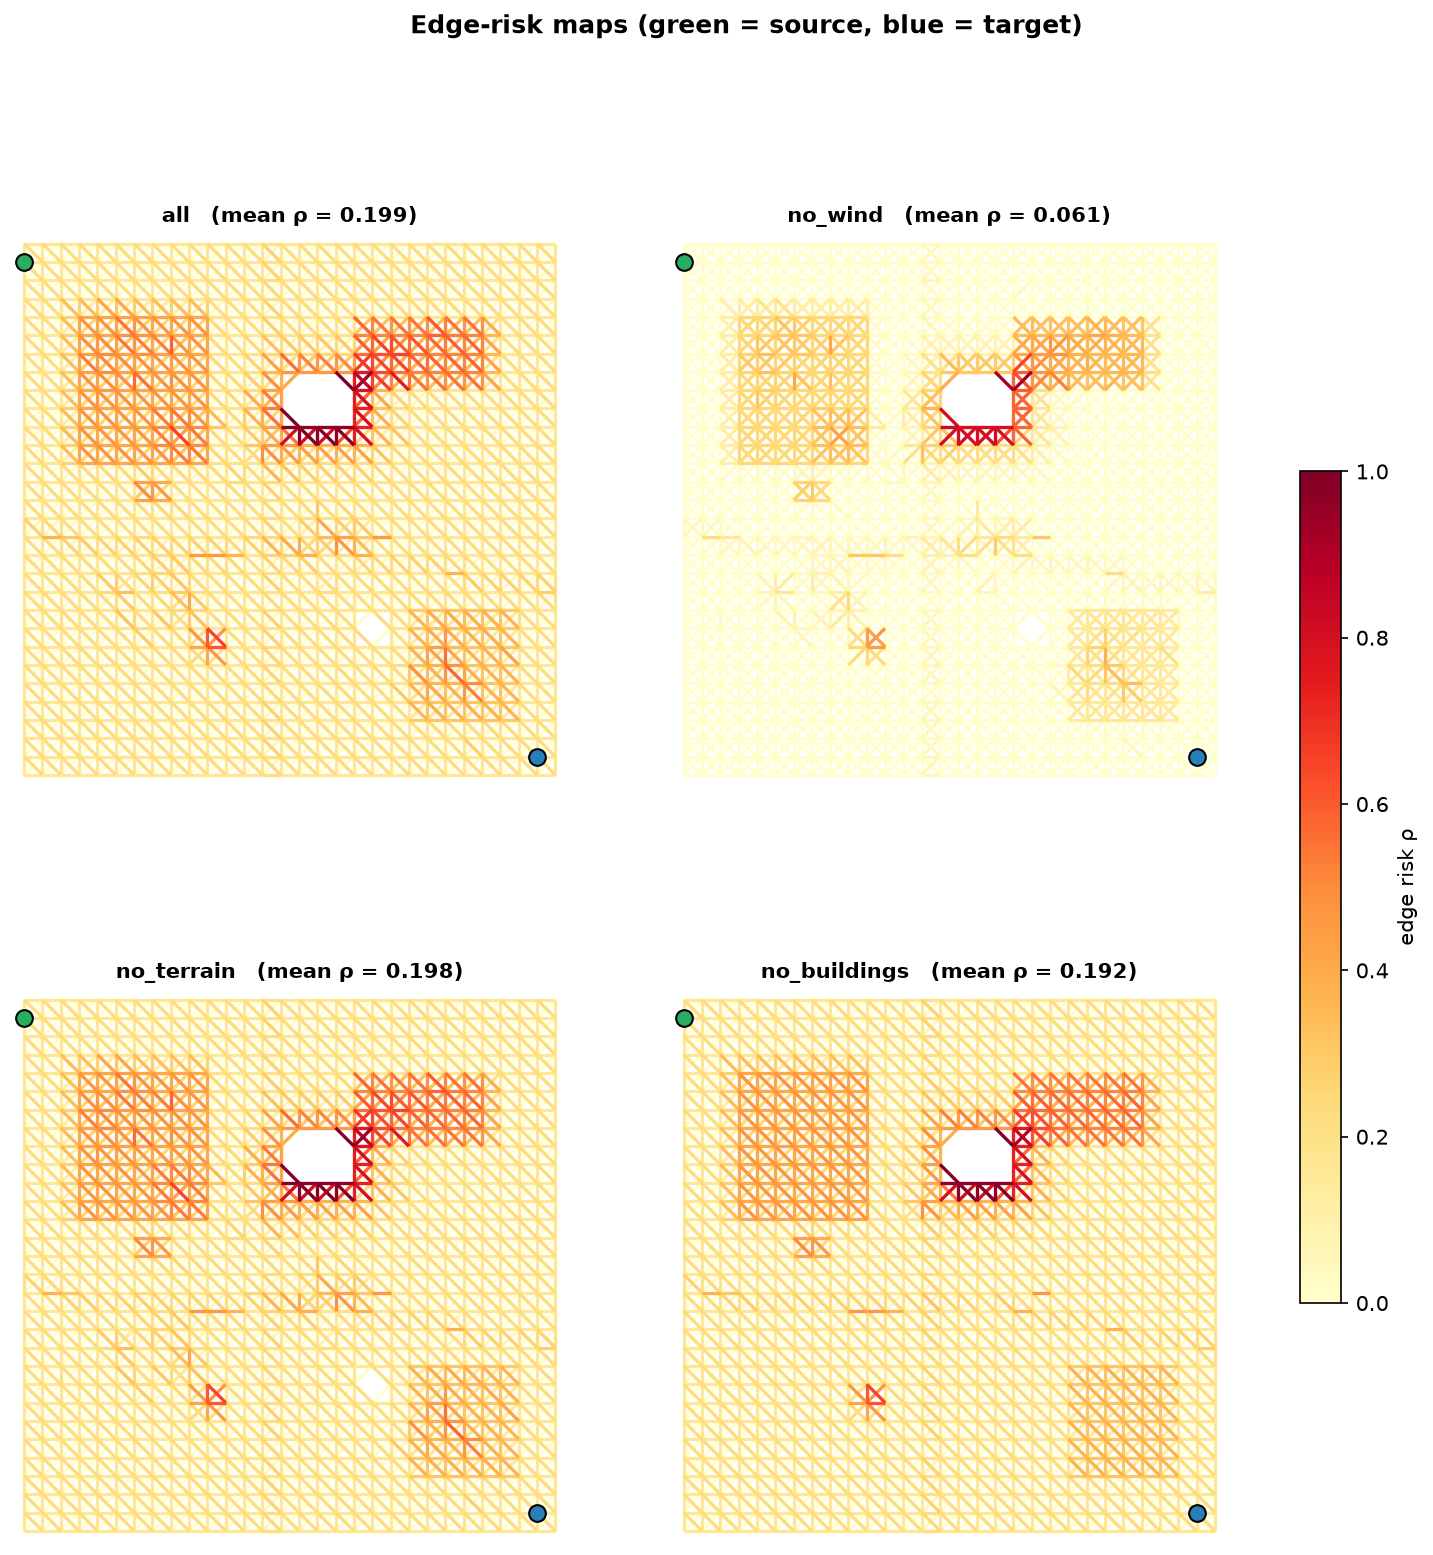
\includegraphics[width=0.85\textwidth]{edge_risk_maps.png}
\caption{Edge risk maps for the ablation variants (fixture layers)}\label{fig:risk-maps}
\end{figure}

\section{Tier 2 Selection}

Table~\ref{tab:tier2} shows the Tier~2 picks on the S2 and S3 fronts of the benchmark. The
ranks are the selected route's position on each objective within the front (1 is best).

\begin{table}[H]
\centering\caption{Tier~2 picks on the S2 (16 routes) and S3 (115 routes) fronts; last column is latency in ms}\label{tab:tier2}\footnotesize\setlength{\tabcolsep}{4pt}
\begin{tabular}{l l r r r l r}
\toprule
\textbf{Front} & \textbf{Preset} & \textbf{Rank $d$} & \textbf{Rank $\varepsilon$} & \textbf{Rank $\rho$} & \textbf{Point type} & \textbf{ms}\\
\midrule
\multirow{4}{*}{S2} & Fragile medical    & 7  & 5  & 10 & non-extreme & 0.030\\
                    & Emergency medicine & 3  & 1  & 14 & min-energy  & 0.025\\
                    & Disaster relief    & 3  & 1  & 14 & min-energy  & 0.022\\
                    & Mixed cargo        & 4  & 2  & 13 & non-extreme & 0.023\\
\midrule
\multirow{4}{*}{S3} & Fragile medical    & 91 & 81 & 25 & non-extreme & 0.144\\
                    & Emergency medicine & 22 & 26 & 94 & non-extreme & 0.140\\
                    & Disaster relief    & 28 & 1  & 88 & min-energy  & 0.136\\
                    & Mixed cargo        & 84 & 59 & 32 & non-extreme & 0.136\\
\bottomrule
\end{tabular}
\end{table}

On the 115-route S3 front, three of the four presets select non-extreme points, and the
four presets select four different routes. Disaster relief takes the minimum-energy
route, which matches its dominant weight. The emergency medicine pick is worth a closer
look. It is the 22nd-shortest route, yet it is only 1.9\% longer than the shortest route
on the front. Its weights are dominated by distance, but not completely, so the utility
accepts a very small distance penalty in exchange for a lower risk. A single-objective
planner cannot make that trade, and a fixed-weight planner would make the same trade for
every payload. The fragile medical pick is 25th of 115 in risk rather than first, which
again reflects its non-zero distance and energy weights. Every selection took well under
a millisecond, far inside the one-second target.

On the smaller S2 front the picks are less spread: emergency medicine and disaster
relief share the minimum-energy route, which on this graph is also near the shortest. This
is the same pattern as in the wind experiment, and it points to the size of the front as
the factor that limits how many distinct choices Tier~2 can make.

Figure~\ref{fig:osm-routes} shows the four presets on a 2\,km lattice
with OpenStreetMap roads drawn underneath for reference. The fragile medical and mixed
cargo presets take a slightly longer path (2.6\,km) with a cumulative risk of 1.57, while
emergency medicine and disaster relief take 2.5\,km paths with risks of 1.88 and 1.89.

\begin{figure}[H]
\centering
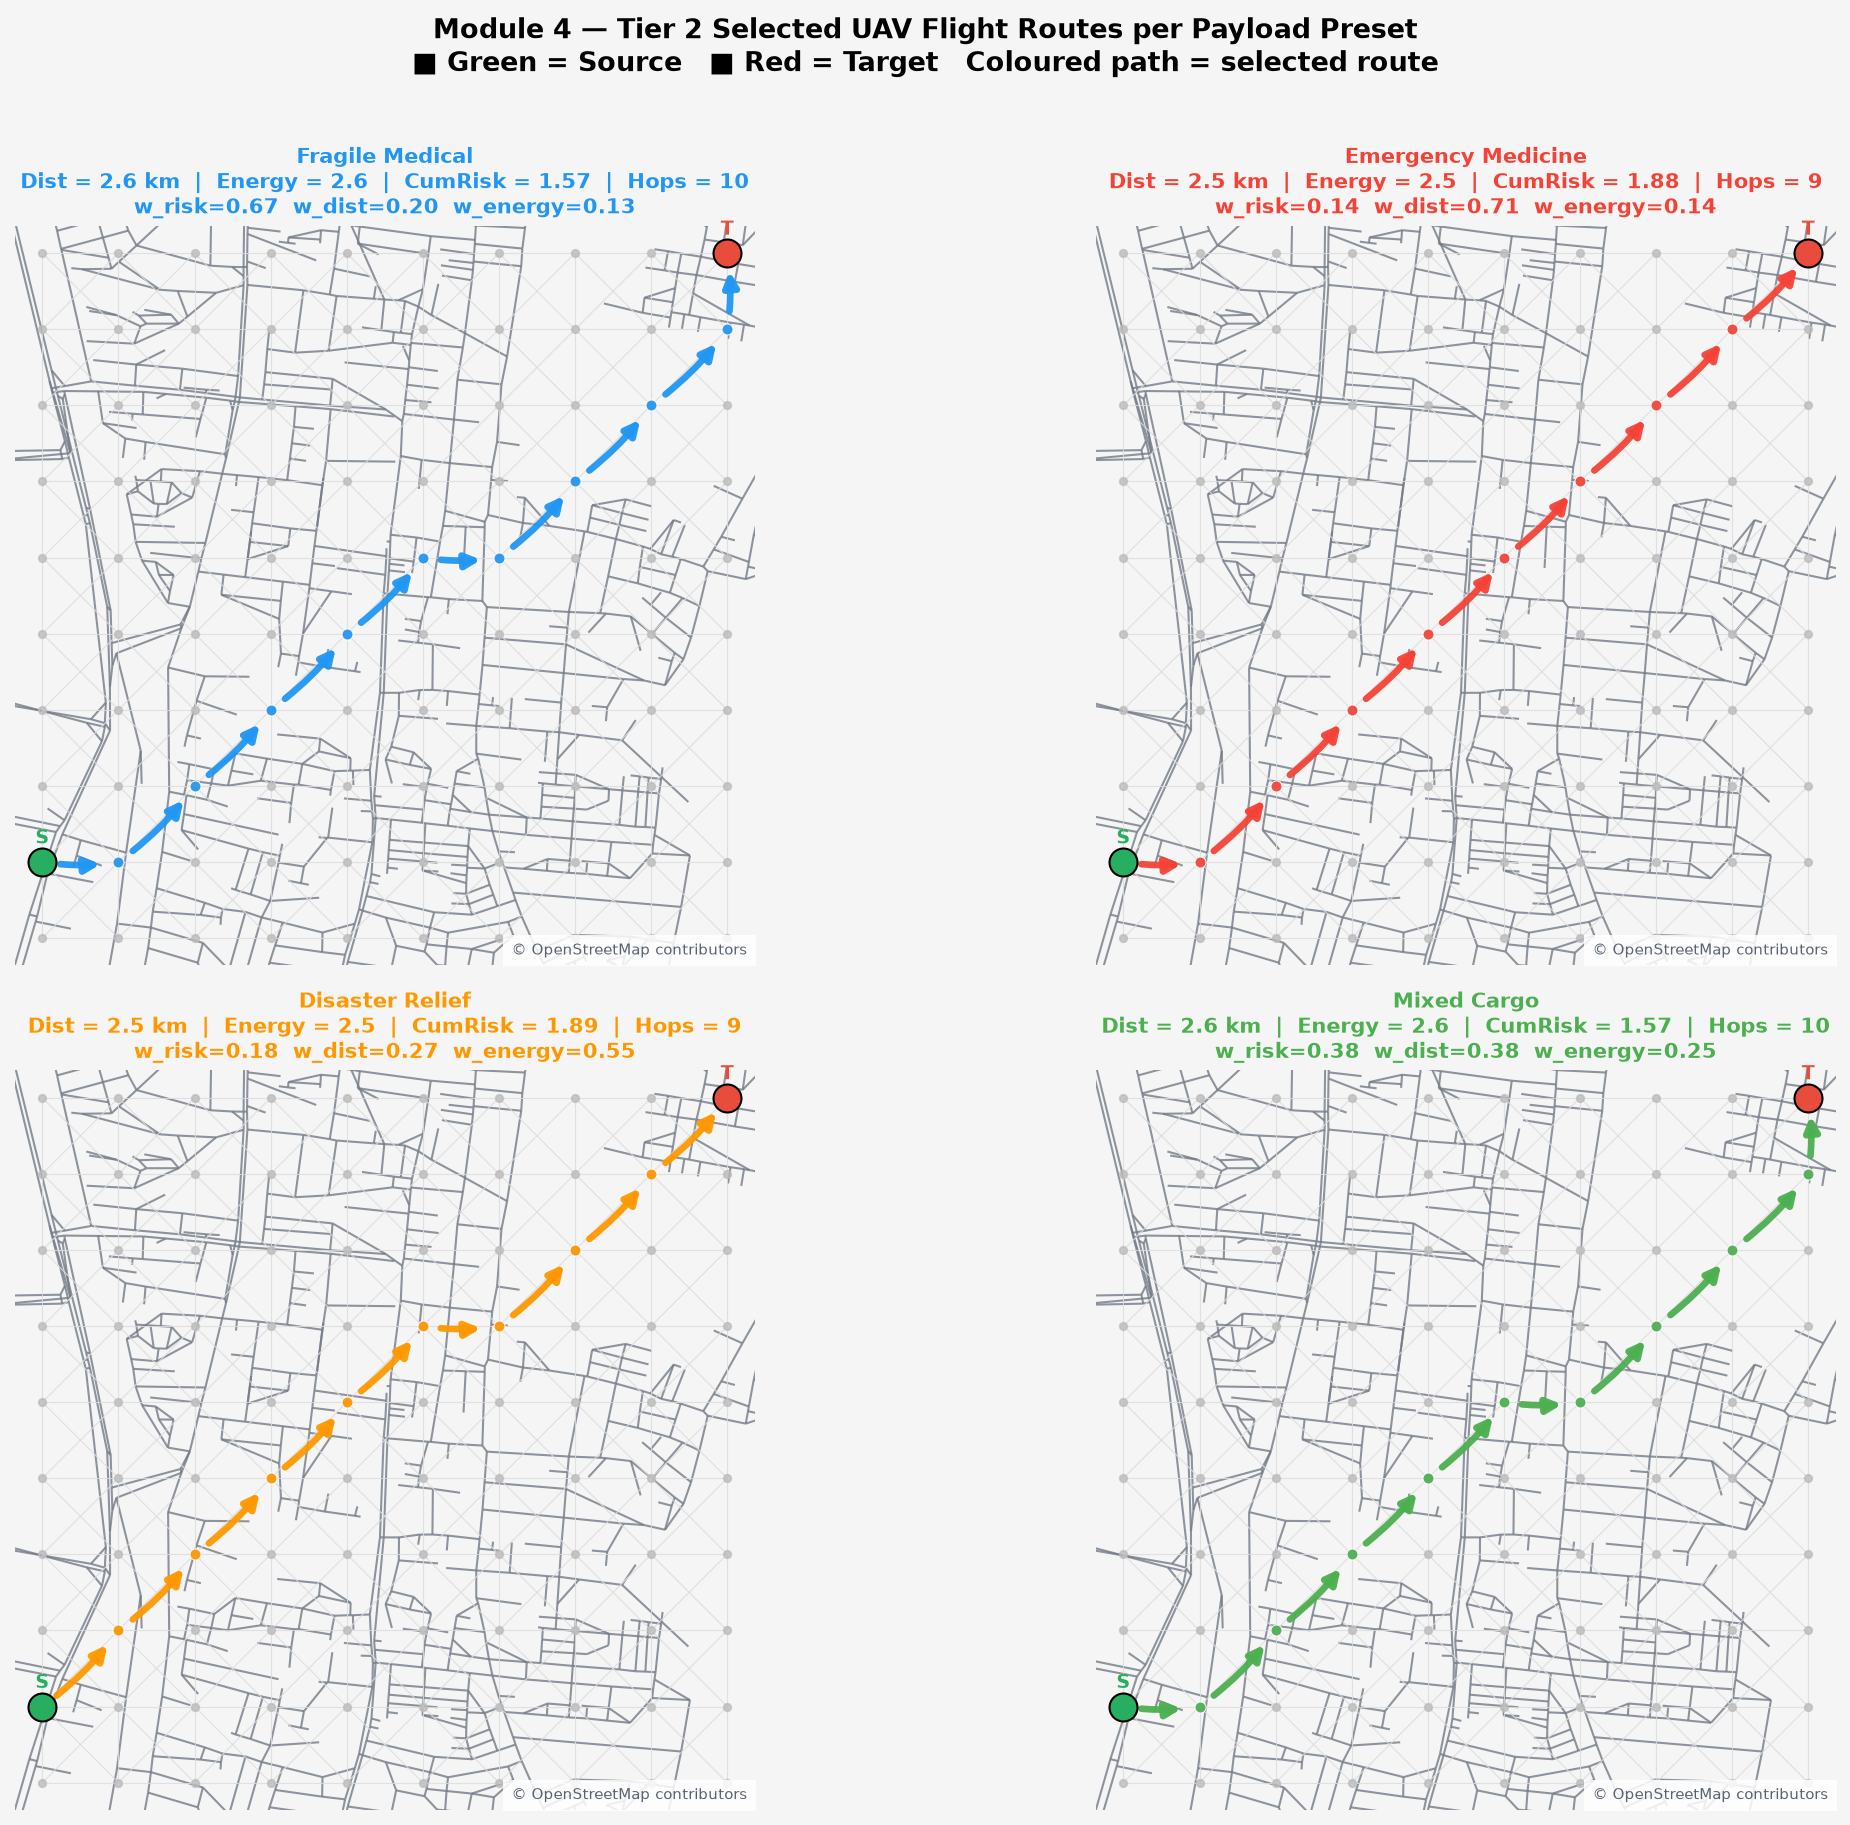
\includegraphics[width=0.92\textwidth]{osm_module4_routes_on_graph.png}
\caption{Tier~2 routes for the four presets on a 2\,km lattice}\label{fig:osm-routes}
\end{figure}

\section{Simulation Results So Far}

The SITL mission runner has been flown against ArduCopter SITL (4.8.0-dev, built-in
quadcopter physics, run at five times real time) with missions produced by the planner
from a fixture bundle. Mission upload, read-back, the switch to AUTO, landing and disarm
all succeeded. The cross-track root-mean-square error between the flown and planned
tracks was 0.11--0.13\,m, and the landing offset from the destination pad was
0.01--0.02\,m. These numbers show that the mission chain from Tier~2 to the autopilot is
correct, including the altitude frame. They do not yet say anything about the city model,
wind in the simulator or the battery, which are the open items listed in
Chapter~\ref{cha:queries}.

\section{Comparison With Existing Work}

Table~\ref{tab:compare} compares the system with the three works reviewed in
Section~\ref{sec:relatedwork}.

\footnotesize
\begin{xltabular}{\textwidth}{L{2.5cm} Y Y Y Y}
\caption{Comparison with the reviewed works}\label{tab:compare}\\
\toprule
\textbf{Property} & \textbf{Chokkalingam \& Ganesan \cite{r1}} & \textbf{Tsoutsouras et al.\ \cite{r10}} & \textbf{Ren et al.\ \cite{r3}} & \textbf{This work}\\
\midrule
\endfirsthead
\multicolumn{5}{l}{\small\itshape Table \thetable\ (continued)}\\
\toprule
\textbf{Property} & \textbf{Chokkalingam \& Ganesan \cite{r1}} & \textbf{Tsoutsouras et al.\ \cite{r10}} & \textbf{Ren et al.\ \cite{r3}} & \textbf{This work}\\
\midrule
\endhead
\bottomrule
\endlastfoot
Front construction & POPSO, stochastic & None & CDNSGA-II, stochastic & NAMOA*, exact and deterministic\\
Objectives & Multiple, scalarised for the final pick & Energy and speed & Distance, safety & Distance, energy, risk\\
Final route selection & Weighted sum, weights tuned per mission & Not applicable & Crowding distance & Utility from payload tags, argmax over the full front\\
Payload in selection & No & Mass in the energy model only & No & Fragility, weight class, urgency, priority\\
Wind direction in edge costs & Not reported & Not reported & Not reported & Headwind and crosswind per edge, gust, shear, weather gate\\
Front reuse & Re-run per mission & Not applicable & Re-run per mission & Stored front with drift-based refresh\\
\end{xltabular}
\normalsize

The comparison is qualitative for now. Their datasets and code are not public, so the
quantitative comparison uses the selection rules they describe (crowding distance as in
Ren et al., fixed weights as in Chokkalingam and Ganesan) applied to our fronts, through
the payload-alignment score of Section~\ref{sec:m5}. That comparison runs at report scale
in the next pass.

\section{Discussion and Next Steps}

So far the results support a few claims. The exact Tier~1 front covers the reference front
completely while MOPSO recovers a third of it on the largest scenario. Tier~2 picks
non-extreme routes for mixed payloads in well under a millisecond, and on a large front
different payloads get different routes. The directional wind model changes energy, risk
and the shape of the front in the way the physics predicts, and a direction-blind model
would miss a 27.5\% energy difference at a fixed wind speed.

They also expose what the next passes must fix. The MOPSO comparison needs the
report-scale settings and per-repetition statistics. The density labels must reach the
graph builder. The monotonicity check must be grouped by scenario. The collapse of the
front under steady wind needs a study of normalisation and possibly of the weight
multipliers. The ablation and the Tier~2 results must be repeated on live OpenStreetMap
data, and the risk weights and battery constants must be calibrated. On the simulation
side, the Gazebo world, wind in the simulator and repeated flights per preset come next.
Each of these feeds the cycle described in Chapter~\ref{cha:queries}.


% ============================================================
\bibliography{references}

\end{document}
